\chapter{Computational study}
\label{chap:computational_study}
This chapter will give the most insights into the functionality and efficiency of the usage of the presented binary classifier in
\gls{3L-CVRP} algorithms. This chapter will begin with the selection of two published \gls{3L-CVRP} datasets.
Afterwards the results from the model training are presented, which
is divided in three main parts, firstly the results of the retrieval of the data, secondly the feature selection, and finally presenting
different strategies for comparing different models and selecting the best best fit performance wise.
Afterwards a parameter study is conducted for the \gls{ILS}, starting with the \textit{NoClassifier} variant determining
the best configurations for the base parameters, followed by a variant specific parameter study.
This chapter closes with a computational study of all four variants, comparing the variants with tuned parameters.
These insights are summarized in the concluding chapter.

\section{Comparison of Available Datasets}
\label{sec:dataset_selection}

The \gls{3L-CVRP} is a well-studied problem and several datasets were published in the past, considering
different constraints and characteristics. A selection of these datasets will be compared and evaluated
in this section. The goal is to identify suitable datasets for training a general \gls{CLP} classifier that can predict
the loading feasibility of single tours from different datasets. Therefore, the dataset needs
heterogeneous characterists to represent numerous possible use-cases
as shown in Section~\ref{sec:motivation_feasibility_prediction}. Five published
\cgls{3L-CVRP} datasets are presented with respect to their overall characteristics.
Each dataset gets an unique identfier to simplify the comparison and is shown in parenthesis
after the following individual introduction. The first \cgls{3L-CVRP} dataset was published by \citeauthor{gendreau_tabu_2006} in
\citeyear{gendreau_tabu_2006} and delivered the first \cgls{3L-CVRP} instances containing huge and heavy items (\gendreauDataSet).\footcite[cf.][]{gendreau_tabu_2006}
The second dataset was published by \citeauthor{moura_integrated_2009} in \citeyear{moura_integrated_2009},
and combines the \gls{VRP} from \citeauthor{solomon_algorithms_1987} and the \gls{CLP} instances from
\citeauthor{bischoff_issues_1995} defining the \gls{3L-VRPTW} considering
many items of small size and weight (\mouraDataSet).\footcites[cf.][]{solomon_algorithms_1987,bischoff_issues_1995}[][]{moura_integrated_2009}
The first dataset containing real-life data was published by \citeauthor{ceschia_local_2013} in \citeyear{ceschia_local_2013}
and contains the instances with the most items (\ceschiaDataSet).\footcite[cf.][]{ceschia_local_2013}
Krebs published two different datasets in
\citeyear{krebs_advanced_2021} with a focus on more realistic constraints. The first one contains a set
of realistic constraints and offers a wide range of instance sizes (\krebsADataSet).\footcite[cf.][]{krebs_advanced_2021}
The second one focuses on semi-trailer trucks and special requirements for axle weights (\krebsBDataSet).\footcite[cf.][]{krebs_axle_2021}
The characteristics of the datasets are summarized in the following Table~\ref{tab:dataset_comparison},
where the brackets [\,] indicate a range of possible values. All values considering mass and volume are
\textit{relative} to the respective vehicle weight and volume limit to be comparable. A \textit{item type} is
defined by its geometrical dimensions, the weight, and possible stability characteristics, such as fragility or \gls{LBS}.
When the number of item types is smaller than the number of items equal item types occur multiple times. The types column
depict the number of different item types per instance. Additionaly
most features of the dataset are compared with \textit{aggregated}  values, referring to the aggregrated characteristics
of all items requested by one customer, so the aggregated mass, volume and items shows the average value requested by an
customer of this dataset.

\newcolumntype{C}[1]{>{\centering\arraybackslash}p{#1}}
\newcolumntype{L}[1]{>{\raggedright\arraybackslash}p{#1}} % left-aligned
\begin{table}[ht]
    \centering
    \small
    \renewcommand{\arraystretch}{1.1}   % a touch more row height
    \begin{tabular}{@{}lccccc@{}}
        \toprule
        \textbf{Dataset} & \textbf{Instances} & \textbf{Customers} & \textbf{Agg. Mass}\footnote{Average is based on all customers of the instances.} & \textbf{Agg. Vol.} \footnotemark[\value{footnote}]       & \textbf{Agg. Items}\footnotemark[\value{footnote}] \\
        \midrule
        \gendreauDataSet & 27                 & [15, 100]          & 0.137                                                                            & 0.127                                                    & 2.00                                               \\
        \mouraDataSet    & 46                 & 25                 & 0.077                                                                            & 0.176                                                    & 52.0                                               \\
        \ceschiaDataSet  & 13                 & [11, 129]          & 0.063                                                                            & 0.160                                                    & 18.1                                               \\
        \krebsADataSet   & 600                & [20, 100]          & 0.098                                                                            & 0.100                                                    & 4.41                                               \\
        \krebsBDataSet   & 80                 & [30, 120]          & 0.036                                                                            & 0.052                                                    & 4.00                                               \\
        \toprule
        \textbf{Dataset} & \textbf{Items}     & \textbf{Types}     & \textbf{\text{Routes}}\footnote{Average is based on the instances.}              & \textbf{\text{Route Len}}\footnotemark[\value{footnote}] & \textbf{Fragility}\footnotemark[\value{footnote}]  \\
        \midrule
        \gendreauDataSet & [26, 199]          & [26, 199]          & 6.13                                                                             & 6.22                                                     & 0.25                                               \\
        \mouraDataSet    & 1050, 1550         & 5                  & 4.40                                                                             & 6.72                                                     & 0.29                                               \\
        \ceschiaDataSet  & [254, 8060]        & [9, 97]            & 10.2                                                                             & 5.81                                                     & 0.10                                               \\
        \krebsADataSet   & 200, 400           & 3, 10, 100         & 6.77                                                                             & 13.6                                                     & 0.24                                               \\
        \krebsBDataSet   & 200, 400           & 10, 100            & 3.87                                                                             & 22.1                                                     & 0.10                                               \\
        \bottomrule
    \end{tabular}
    \caption[Numerical comparison of different 3L--CVRP Datasets.]{Numeric comparisons between five avalaible datasets.}
    \label{tab:dataset_comparison}
\end{table}

The columns routes, route length and fragility show the average over all instances.
Routes define the \gls{LB} for the needed vehicles $K$ and route length the average number of customers per route based
on the relative volume and mass. The averages are displayed to become a better understanding of the
statistics of each dataset, rather than looking at extreme values.
The most important consideration, when selecting a suitable dataset for the training of a classifier,
is how representative single tours from one dataset are for all other datasets. Therefore, the numeric characteristics
should not contain outliers. It is apparent, that the \gendreauDataSetText dataset has the least items per customer
with huge relative volume and weight, which leads with an average route length of 6.22 customers to very few items
considered per route in comparison to the other datasets. This makes it easier to compute the feasibility of the loading
as the combinations of placing patterns is limited. The \mouraDataSetText dataset has the most items per average per customer consisting
of only 5 item types. The \ceschiaDataSetText dataset contains the fewest instances, but with the most maximum items of 8060,
which lead to many routes on average. The two datasets from Krebs, have similar
boundaries and values, but \krebsBDataSetText has routes with twice as many customers as \krebsADataSetText on average due
to the smaller average aggregated mass and volume. Both \krebsADataSetText and \gendreauDataSetText
show a good variety of the features, without including too many items per route in comparison to the other datasets.
However, as the average route length from \krebsADataSetText is twice as long and the number of items per customer contain twicw as many,
one route contain per average four times more items leading to a higher complexity for solving the \gls{CLP}.
The following Table~\ref{tab:constraint_matrix} provides an overview of the constraints considered
in each dataset showcasing the realistic profile. The constraints are categorized in the five loading constraint groups introduced
in Section~\ref{sec:clp_definition}.
\clearpage

\begin{table}[ht]
    \centering
    \small
    \renewcommand{\arraystretch}{1.2}
    \begin{tabular}{@{}L{1.8cm}L{3cm}C{1.6cm}C{1.6cm}C{1.6cm}C{1.6cm}C{1.6cm}@{}}
        \toprule
        \textbf{Category}          & \textbf{Constraint} &                        &                     & \textbf{Dataset}      &                      &                      \\
                                   &                     & Gendreau\newline(2006) & Moura\newline(2009) & Ceschia\newline(2013) & Krebs\newline(2021a) & Krebs\newline(2021b) \\
        \midrule
        \multirow{3}{*}{Container} & Load Capacity       & $\bullet$              & $\bullet$           & $\bullet$             & $\bullet$            & $\bullet$            \\
                                   & Load Balance        &                        &                     &                       & $\bullet$            &                      \\
                                   & Axle Weights        &                        &                     &                       & $\bullet$            & $\bullet$            \\\midrule
        \multirow{3}{*}{Item}      & z-Rotation          & $\bullet$              & $\bullet$           & $\bullet$             & $\bullet$            & $\bullet$            \\
                                   & Fragility           & $\bullet$              &                     & $\bullet$             & $\bullet$            & $\bullet$            \\
                                   & LBS                 &                        &                     & $\bullet$             & $\bullet$            &                      \\\midrule
        \multirow{1}{*}{Cargo}     & Complete Shipm.     & $\bullet$              & $\bullet$           &                       & $\bullet$            & $\bullet$            \\\midrule
        \multirow{6}{*}{Position}  & Geometry            & $\bullet$              & $\bullet$           & $\bullet$             & $\bullet$            & $\bullet$            \\
                                   & Orthogonality       & $\bullet$              & $\bullet$           & $\bullet$             & $\bullet$            & $\bullet$            \\
                                   & Reachability        &                        &                     & $\bullet$             & $\bullet$            &                      \\
                                   & Sequence            & $\bullet$              &                     &                       & $\bullet$            &                      \\
                                   & LIFO                & $\bullet$              & $\bullet$           & $\bullet$             & $\bullet$            & $\bullet$            \\
                                   & MLIFO               &                        &                     & $\bullet$             & $\bullet$            &                      \\\midrule
        \multirow{2}{*}{Load}      & Robust Stability    &                        &                     & $\bullet$             & $\bullet$            &                      \\
                                   & Support Area        & $\bullet$              & $\bullet$           &                       &                      & $\bullet$            \\

        \bottomrule
    \end{tabular}
    \caption[Overview of CLP constraints in selected 3L--CVRP datasets.]{Matrix overview of constraints covered in selected datasets. A bullet ($\bullet$) indicates that the constraint is considered.}
    \label{tab:constraint_matrix}
\end{table}

This comparison shows that all datasets include similar types of constraints, but the level
of complexity varies. \krebsADataSetText and \ceschiaDataSetText stand out by incorporating
more advanced constraints such as robust stability, reachability, and \gls{LBS}, in comparison to
basic ones like support area, \gls{LIFO} and fragility. To further investigate the differences
between the datasets, Figure~\ref{fig:dataset_comparison} visualizes the aggregated relative mass and
volume of all items requested by individual customers.
Additionally, the size of each scatter point indicates the total number of items requested.
For example, the \mouraDataSetText dataset includes 46
instances with 25 customers each, resulting in $25 \cdot 46 = 1150$ dots in the plot.

\begin{figure}[ht]
    \centering
    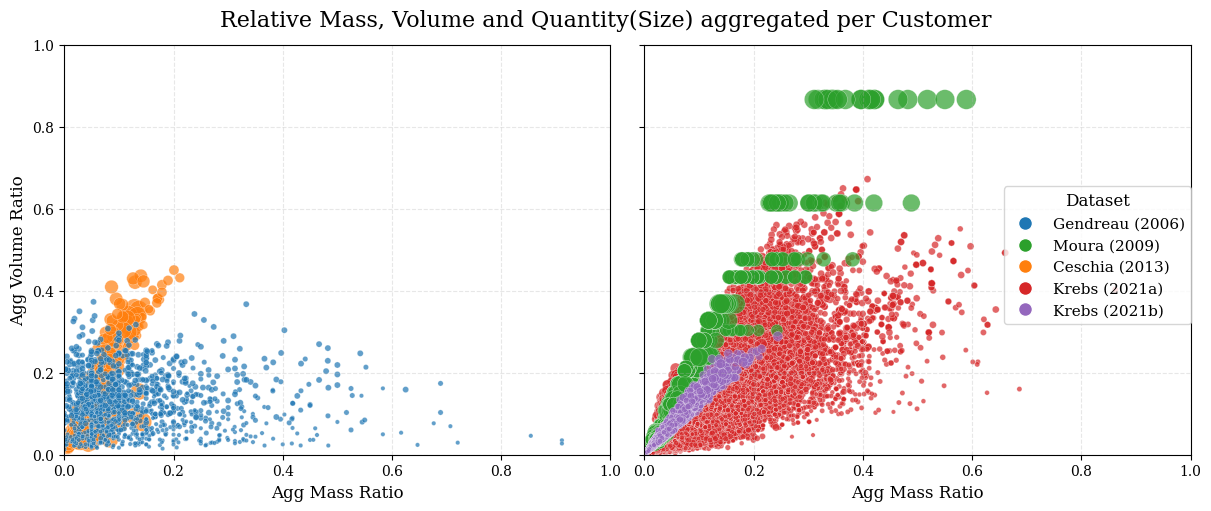
\includegraphics[width=0.85\textwidth]{pictures/comparison_datasets_3lcvrp.png}
    \caption{Comparison aggregated customer demands of different 3L--CVRP/ 3L--VRPTW datasets.}
    \label{fig:dataset_comparison}
\end{figure}

The dispersion of the data points reflects the diversity of individual instances in terms of volume
and mass dependency. A more balanced profile suggests that some customers tend to order items that
are either mass- or volume-intensive, which supports training the model on more heterogeneous data.
Therefore, the dataset should cover a wide range of cases, varying in mass, volume, and item
quantity per customer. The widest spread is observed in \krebsADataSetText and \gendreauDataSetText serving
both as good dataset candidates for training a classifier. Both datasets are investigated further in
the next section.

\section{Analsis of datasets}
\label{sec:analysis_datasets}

The two datasets, \krebsADataSetText and \gendreauDataSet, have a good diverse profile for training
a binary classifier and to be further analyzed.
As shown in Section~\ref{sec:literature_overview} several publications solved the \gendreauDataSetText dataset
with various heuristics and even exact approaches, whereas only one heuristic solution approach exists for the instances of \krebsADataSet.
Both datasets are further analysed in this section to understand dataset specific properties.

\subsubsection{\krebsADataSetText}

The dataset contains 600 instances with 18 instance types derived from the combinations
of number of customers, item types and items. The following Figure~\ref{fig:krebs_dataset_analysis_detailes} plots
the relative mass and volume of all items requested by individual customers for each of the instances. Every color
represents one instance type and the plots are divided by the number of respective customers in three groups, presenting
6 combinations each. There are three levels for the different item types per [3,10,100] and two levels for the total
number of items, 200 and 400, per instance.
\begin{figure}[ht]
    \centering
    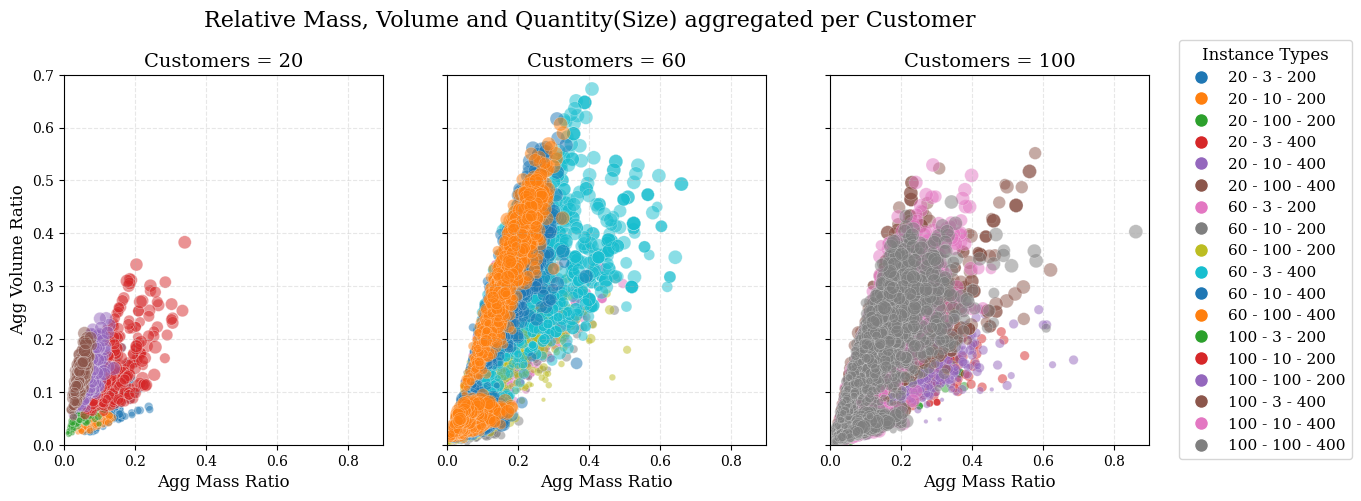
\includegraphics[width=0.85\textwidth]{pictures/krebs_instances_detailed.png}
    \caption[Visualization of different instances of \textcite{krebs_advanced_2021} dataset.]{Visualization of different instances of \krebsADataSetText dataset.
        The instances are named by the number of customers, item types and items.}
    \label{fig:krebs_dataset_analysis_detailes}
\end{figure}%
Several insights can be obtained from the analysis of this plot. Firstly, the aggregated relative
volume and mass per customer is significantly lower for the group with 20 customers than for the groups with 60 or 100 customers.
Secondly, the distribution differs from each instance type, ranging from quite linear distributions in a narrow
interval (e.g. instance 60-100-400) to quite broad distributions (e.g. instance 100-100-400). These two observations need to be considered,
when selecting instances to generate the training data for the classifier to avoid a homogenous training sets.
The instance set should be drawn from every group equally and different distributions need to be considered per group,
that the average numeric route structure differs.

\subsubsection{\gendreauDataSetText}

This dataset consists of 27 instances, where the dispersion of the aggregated mass per customer is reaching very high values, up to
0.91, but has modest volume levels, with a maximum of 0.4 approximately, as could be seen in Figure~\ref{fig:dataset_comparison}. The
following Figure~\ref{fig:aggregated_gendreau_plots} show this dispersion per instance revealing an important insight about the dataset.
As the relative volume is quite for all instances, the relative mass differs between the instances. As it was analyzed from \cite{tamke_branch-and-cut_2024}
the complexity to solve the instances is far greater, when the items are more lightweight and the volume is the limiting factor
for packing items in the container. Furthermore, the authors distinguished the instances in a group of heavy items ($\mathcal{H}$) and
a group of lighweight items ($\mathcal{L}$) by dividing the two groups by the average weight utilization $\overline{\omega}$.\footcite[cf.][pp. 23-25]{tamke_branch-and-cut_2024}
As this classification is based on the optimal solutions, in this thesis another approach will be followed to distinguish both
\krebsADataSetText and \gendreauDataSetText in heavy (H) and lightweight (L) items. An instance is accounted as heavyweigt, if
the average weight aggregated per customer is above the avrage over all instances. This definition has the advantage, that also instances absent
of optimal / good solutions can be labeled. The obtained results for the \gendreauDataSetText and \krebsADataSetText instances will be
differentiated in those two groups to investigate the effect of the average weight per customer on the solution quality and process.

\begin{figure}[ht]
    \centering
    \begin{tikzpicture}[node distance=0mm and 0mm]
        \node[anchor=south, inner sep=0] (A) at (0,0)
        {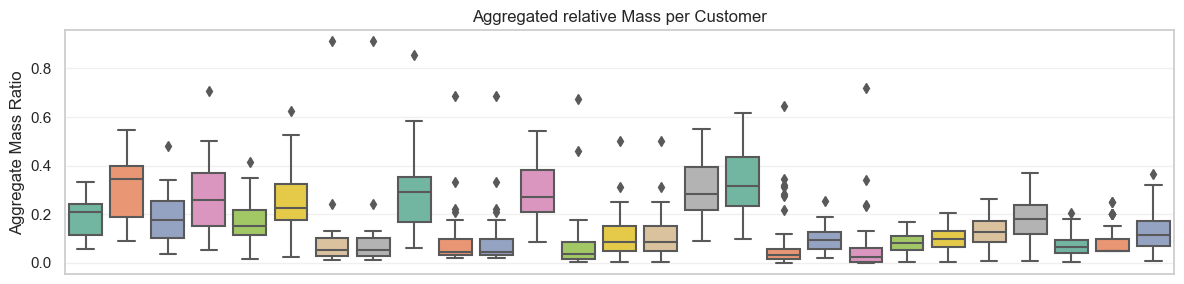
\includegraphics[width=0.95\textwidth]{pictures/AggMassCustGendreau.png}};
        \node[anchor=north, below=of A,inner sep=0] (B)
        {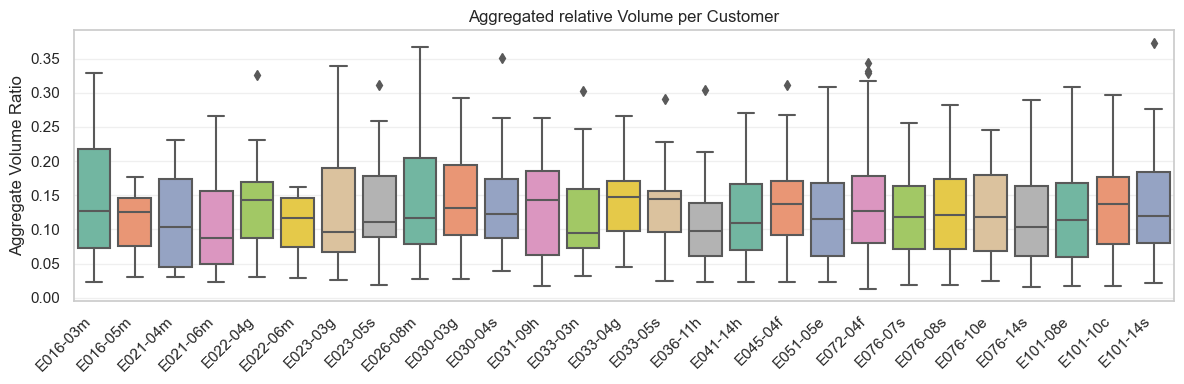
\includegraphics[width=0.96\textwidth]{pictures/AggVolCustGendreau.png}};
    \end{tikzpicture}
    \caption{Aggregated relative mass and volume per customer distributed for each instance of the \gendreauDataSetText dataset.}
    \label{fig:aggregated_gendreau_plots}
\end{figure}

As the construction of train datasets with the \krebsADataSetText is much more computationally challenging as for \gendreauDataSetText,
the following sections will focus only on the latter and the Section~\ref{sec:application_krebs} on solving instances from \krebsADataSet.
Additionally, the Section~\ref{app:sec:krebs_computationally_challenges} in the appendix dives deeper in the challenges for creating a suiting training dataset from the
\krebsADataSetText instances. In the following section the results from training the binary classifier
are presented with diffferent datasets.

\section{Results Training}
\label{sec:ResultsTraining}
In this section the results from the feature dataset selection are discussed. The single best features
with individual scores are shown in the Appendix~\ref{app:feature_selection}. For each model variant (see Section~\ref{sec:modelselection})
the most suiting dataset is selected from both, the Random Retrieval and Save Strategy datasets. These selected
models will then be used in the further steps of the computational study to compare the \gls{ILS} algorithm
with and without the boost of the classifier.

\subsection{Random Retrieval Strategy}
The following random datasets were created with the Algorithm~\ref{fig:flowchart_randomRouteGeneration}.All instances
from \gendreauDataSetText were considered. It must be noted, that the parameter for attempts limit $\beta$ did not have a huge influence on
the number of routes and the structure of the dataset. Therefore only the datasets with $\beta = 30$ have been preselected.
The values in the balance column stand for the share of positive and netative labels in the sample population. The relative volume
and mass refer to the average value for all routes in the respective dataset.

\begin{table}[ht]
    \centering
    \small
    \begin{tabular}{@{}L{0.20\textwidth}P{0.04\textwidth}P{0.04\textwidth}P{0.05\textwidth}P{0.10\textwidth}P{0.12\textwidth}P{0.12\textwidth}P{0.12\textwidth}@{}}
        \toprule
        Name          & $\alpha$           & $\gamma$            & $\delta$ & Routes & Balance   & Rel. Vol & Rel. Mass \\
        \midrule
        RD-2-30-20-6  & \multirow{3}{*}{2} & \multirow{3}{*}{20} & 0.6      & 36779  & 34.4/65.6 & 0.66     & 0.55      \\
        RD-2-30-20-8  &                    &                     & 0.8      & 40724  & 29.0/71.0 & 0.69     & 0.59      \\
        RD-2-30-20-10 &                    &                     & 1        & 47350  & 24.3/75.7 & 0.75     & 0.65      \\
        \midrule
        RD-2-30-30-6  & \multirow{3}{*}{2} & \multirow{3}{*}{30} & 0.6      & 56644  & 33.6/66.4 & 0.66     & 0.55      \\
        RD-2-30-30-8  &                    &                     & 0.8      & 63011  & 28.2/71.8 & 0.69     & 0.59      \\
        RD-2-30-30-10 &                    &                     & 1        & 72408  & 24.2/75.8 & 0.75     & 0.6       \\
        \midrule
        RD-3-30-20-6  & \multirow{3}{*}{3} & \multirow{3}{*}{20} & 0.6      & 48987  & 35.4/64.6 & 0.65     & 0.54      \\
        RD-3-30-20-8  &                    &                     & 0.8      & 61376  & 28.8/71.2 & 0.69     & 0.59      \\
        RD-3-30-20-10 &                    &                     & 1        & 70843  & 24.5/75.5 & 0.74     & 0.64      \\
        \midrule
        RD-3-30-30-6  & \multirow{3}{*}{3} & \multirow{3}{*}{30} & 0.6      & 84751  & 33.8/66.2 & 0.66     & 0.55      \\
        RD-3-30-30-8  &                    &                     & 0.8      & 93942  & 28.6/71.4 & 0.69     & 0.59      \\
        RD-3-30-30-10 &                    &                     & 1        & 108597 & 24.0/76.0 & 0.75     & 0.65      \\
        \midrule
        RD-4-30-20-6  & \multirow{3}{*}{4} & \multirow{3}{*}{20} & 0.6      & 73549  & 34.4/65.6 & 0.66     & 0.55      \\
        RD-4-30-20-8  &                    &                     & 0.8      & 81607  & 28.9/71.1 & 0.69     & 0.59      \\
        RD-4-30-20-10 &                    &                     & 1        & 94666  & 24.2/75.8 & 0.75     & 0.65      \\
        \midrule
        RD-4-30-30-6  & \multirow{3}{*}{4} & \multirow{3}{*}{30} & 0.6      & 113241 & 33.7/66.3 & 0.66     & 0.55      \\
        RD-4-30-30-8  &                    &                     & 0.8      & 125181 & 28.4/71.6 & 0.69     & 0.59      \\
        RD-4-30-30-10 &                    &                     & 1        & 144311 & 24.1/75.9 & 0.75     & 0.65      \\
        \midrule
        RD-5-40-40-6  & \multirow{3}{*}{5} & \multirow{3}{*}{40} & 0.6      & 197525 & 32.0/68.0 & 0.67     & 0.56      \\
        RD-5-40-40-8  &                    &                     & 0.8      & 217085 & 27.3/72.7 & 0.70     & 0.60      \\
        RD-5-40-40-10 &                    &                     & 1        & 249762 & 23.1/76.9 & 0.76     & 0.66      \\
        \bottomrule
    \end{tabular}
    \caption{Created instances for different parameter combinations $(\alpha, \beta, \gamma, \delta)$ for \gendreauDataSetText dataset.}
    \label{tab:created_instances_xyz_gendreau}
\end{table}
The greatest impact on the route characteristics contained in the datasets has parameter $\delta$ as fewer and lighter packed routes
are created. The route characteristics of balance and relative volume and weight are nearly identical for each other tuple combination
of ($\alpha$,$\beta$,$\gamma$). This influence is visualized in the following Figure~\ref{fig:route-dists_randomdata}, where the distribution
of the route length of each $\delta$ variant is shown for an exemplary random dataset.

\begin{figure}[!h]
    \centering
    \begin{subfigure}[t]{.33\textwidth}
        \centering
        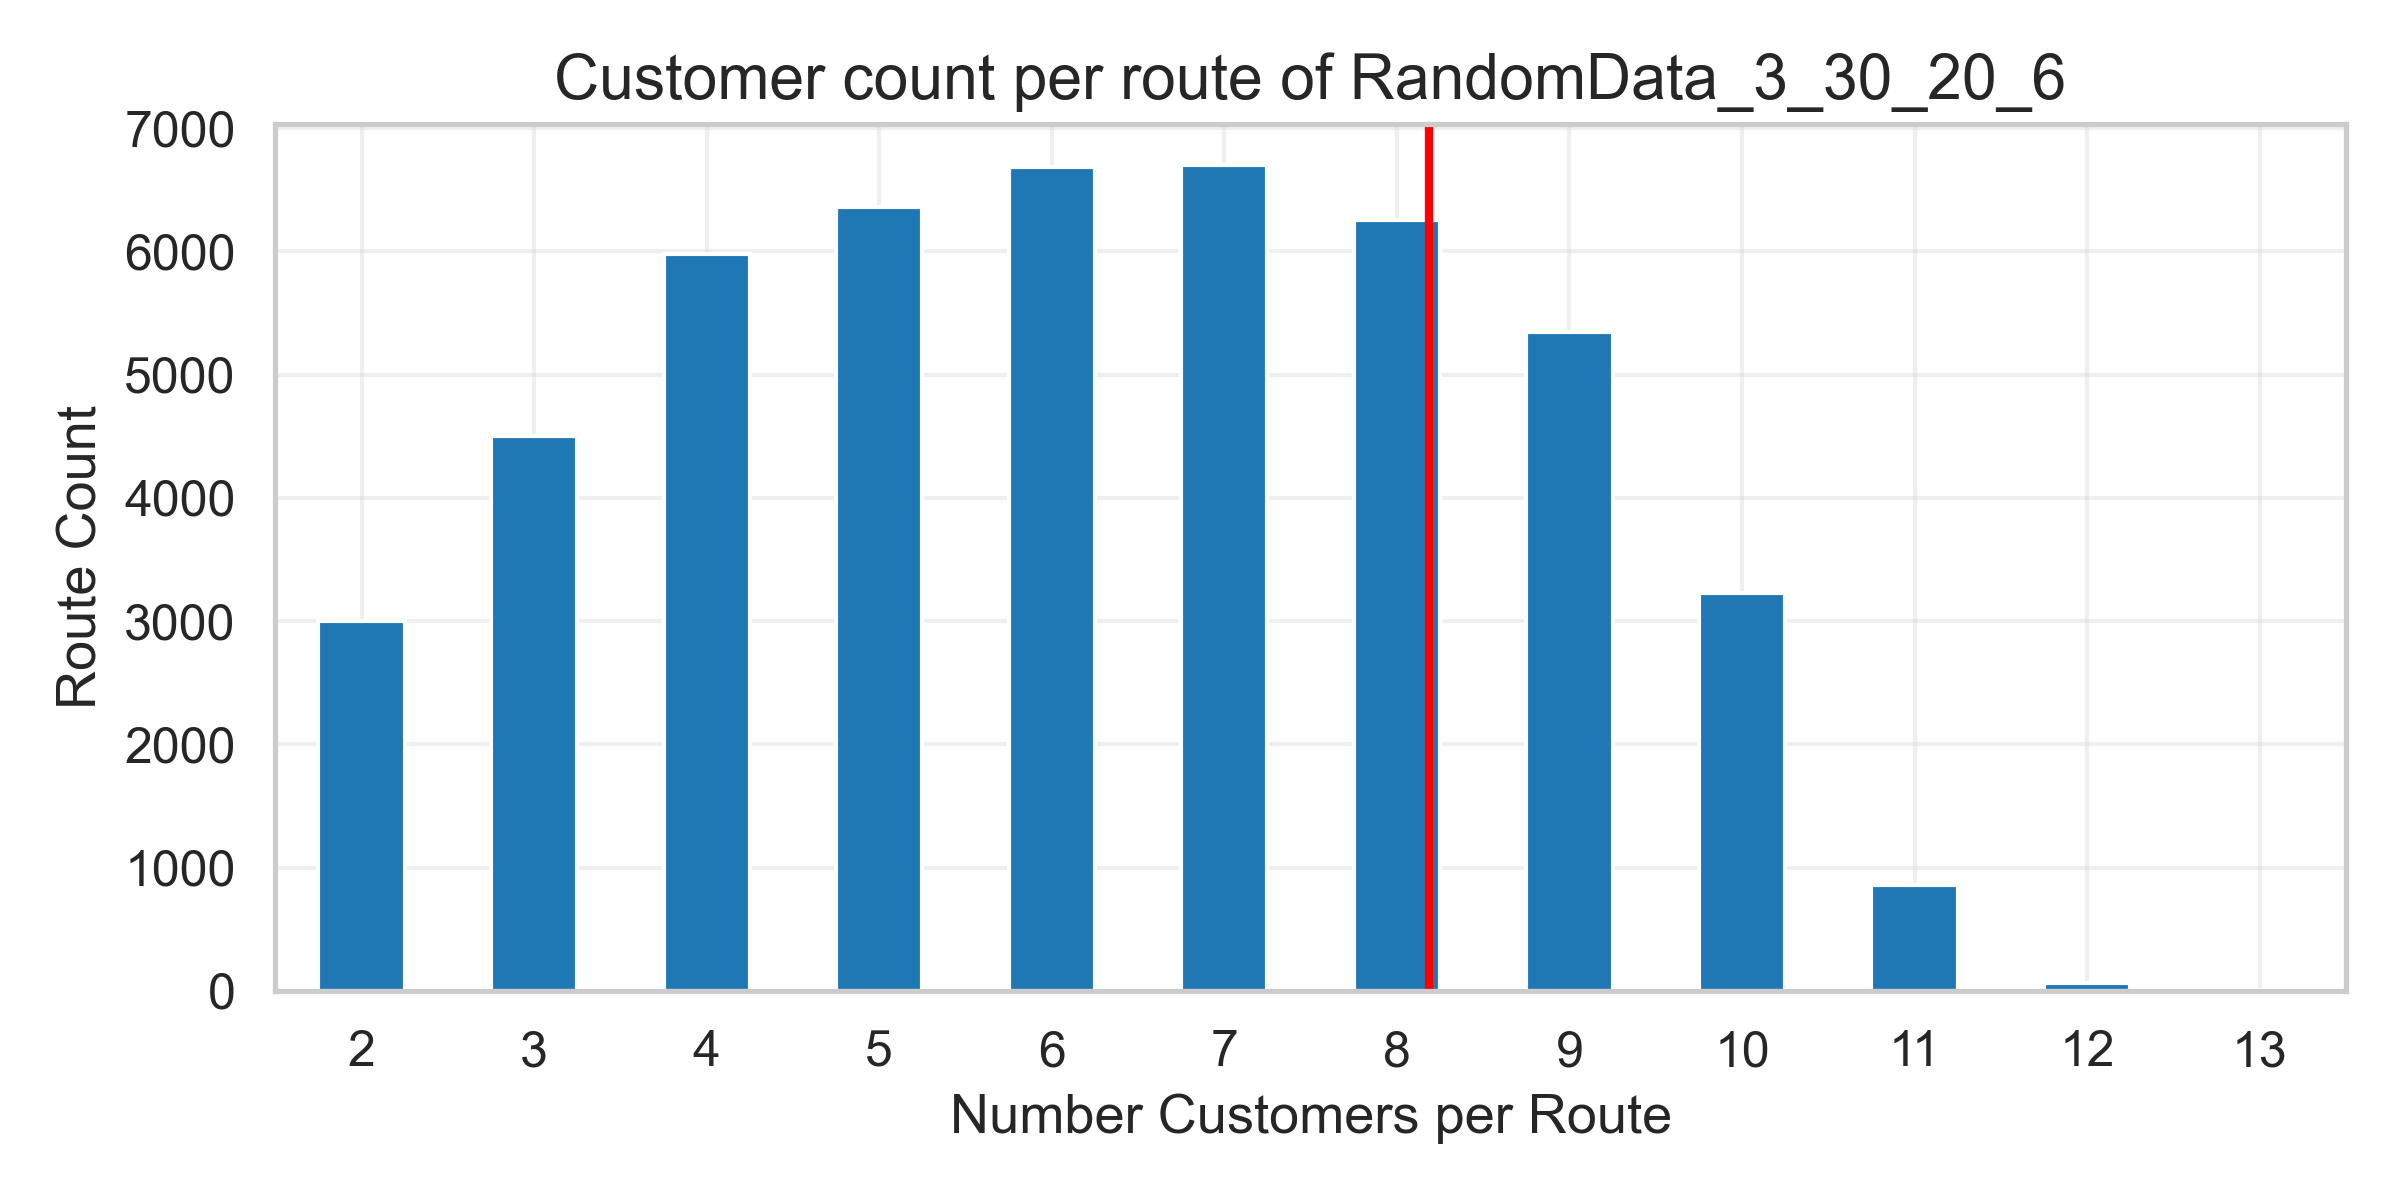
\includegraphics[width=\linewidth]{pictures/dataset_structure/no_cust_plot_RandomData_3_30_20_6.png}
        \caption{RD-3-30-20-6; \\Threshold $\delta$ = 0.6.}
        \label{fig:ds-a}
    \end{subfigure}%
    \begin{subfigure}[t]{.33\textwidth}
        \centering
        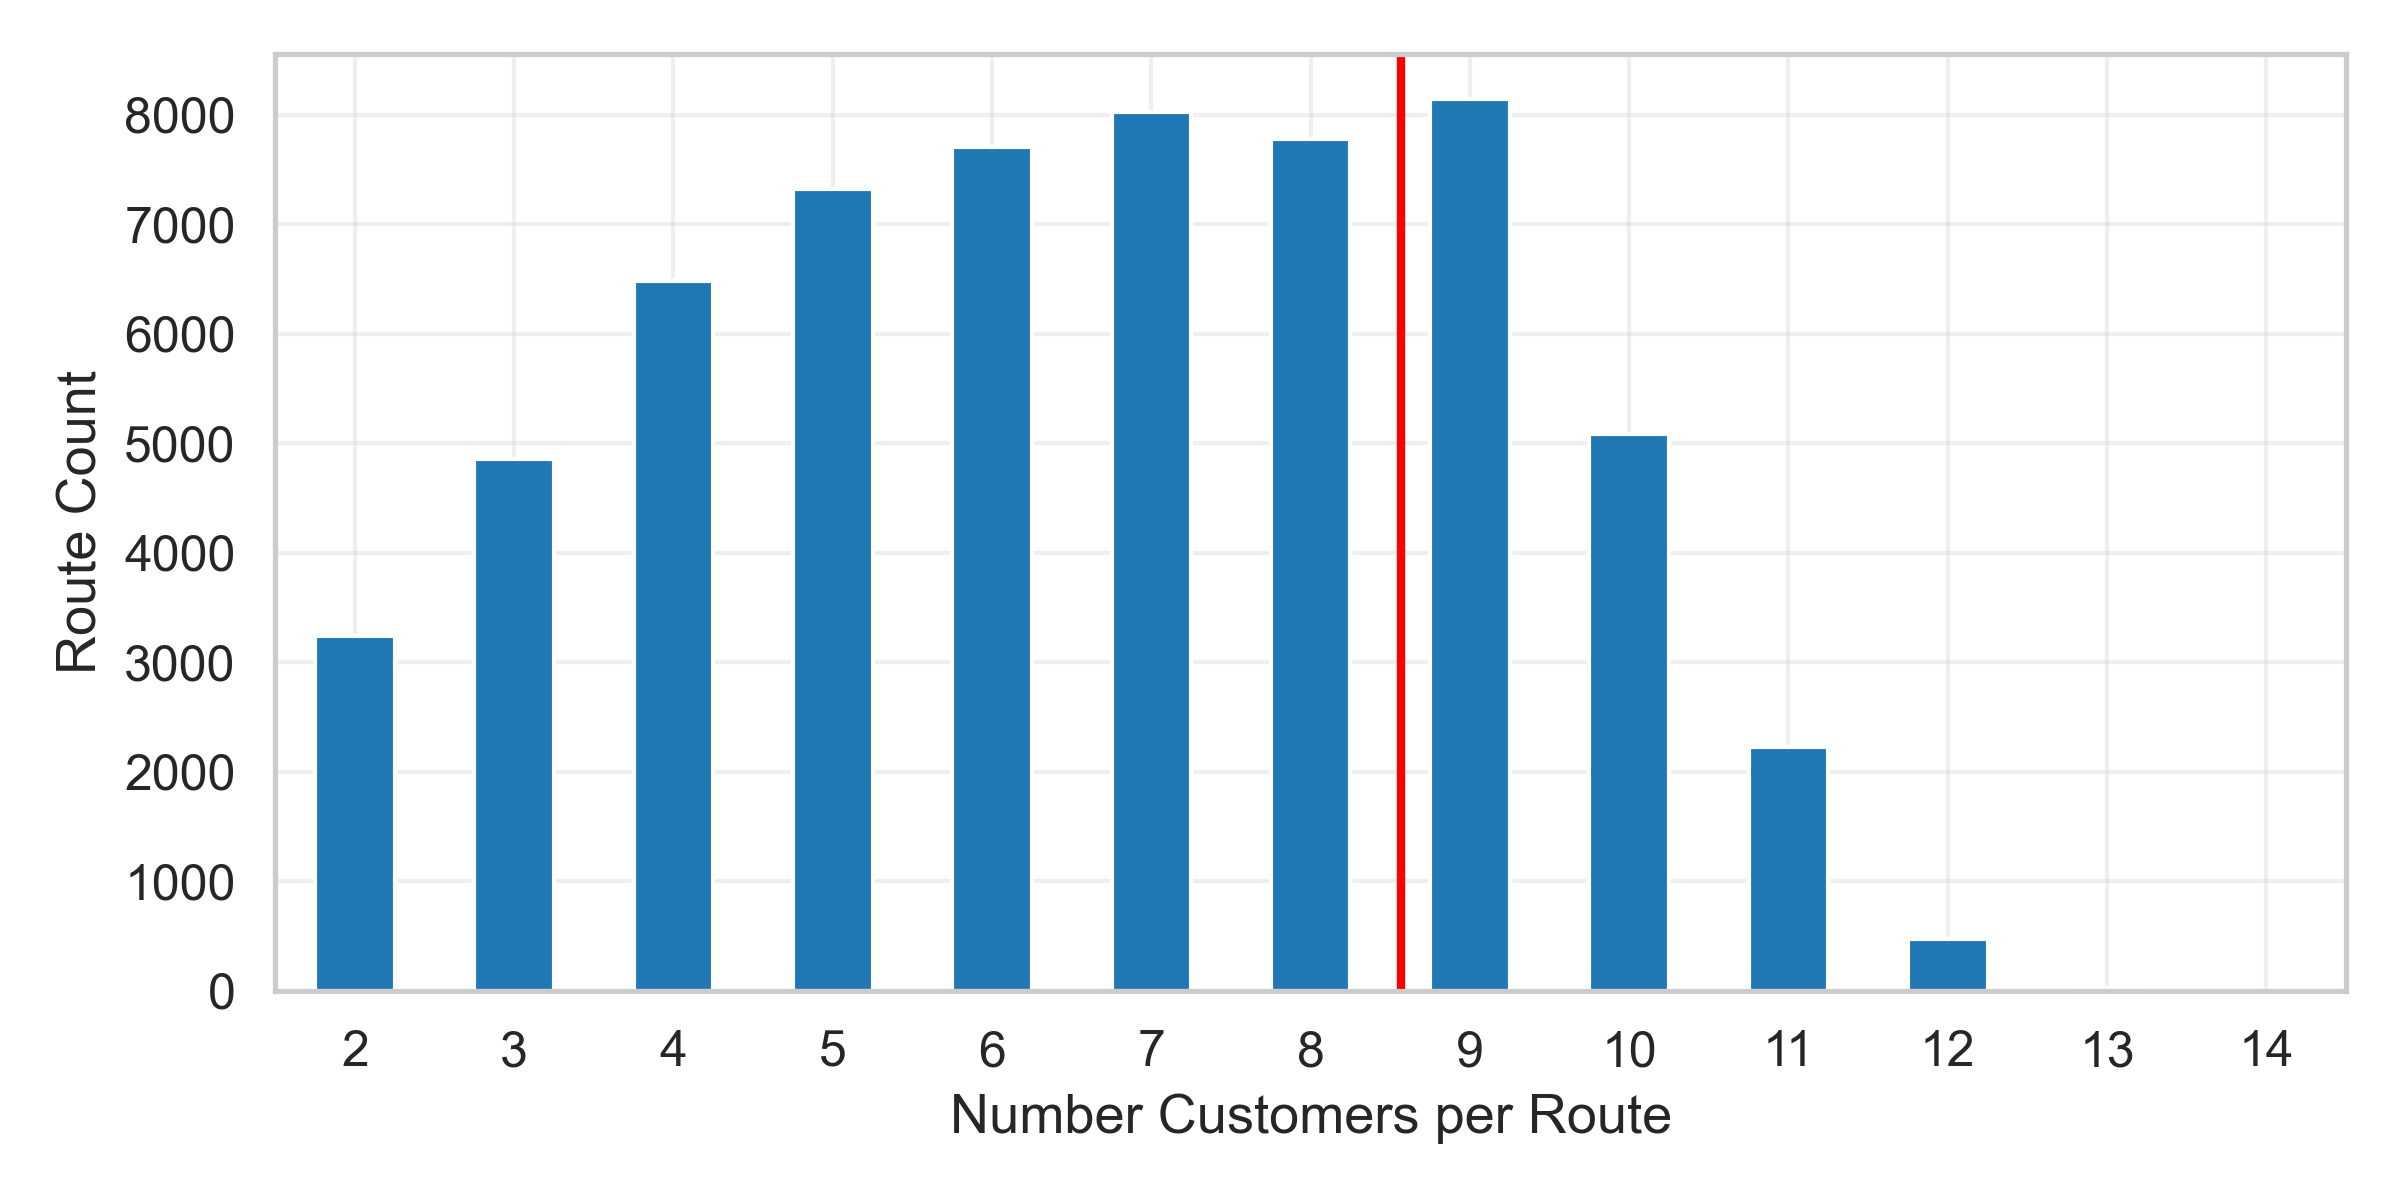
\includegraphics[width=\linewidth]{pictures/dataset_structure/no_cust_plot_RandomData_3_30_20_8.png}
        \caption{RD-3-30-20-8; \\Threshold $\delta$ = 0.8.}
        \label{fig:ds-b}
    \end{subfigure}
    \begin{subfigure}[t]{.33\textwidth}
        \centering
        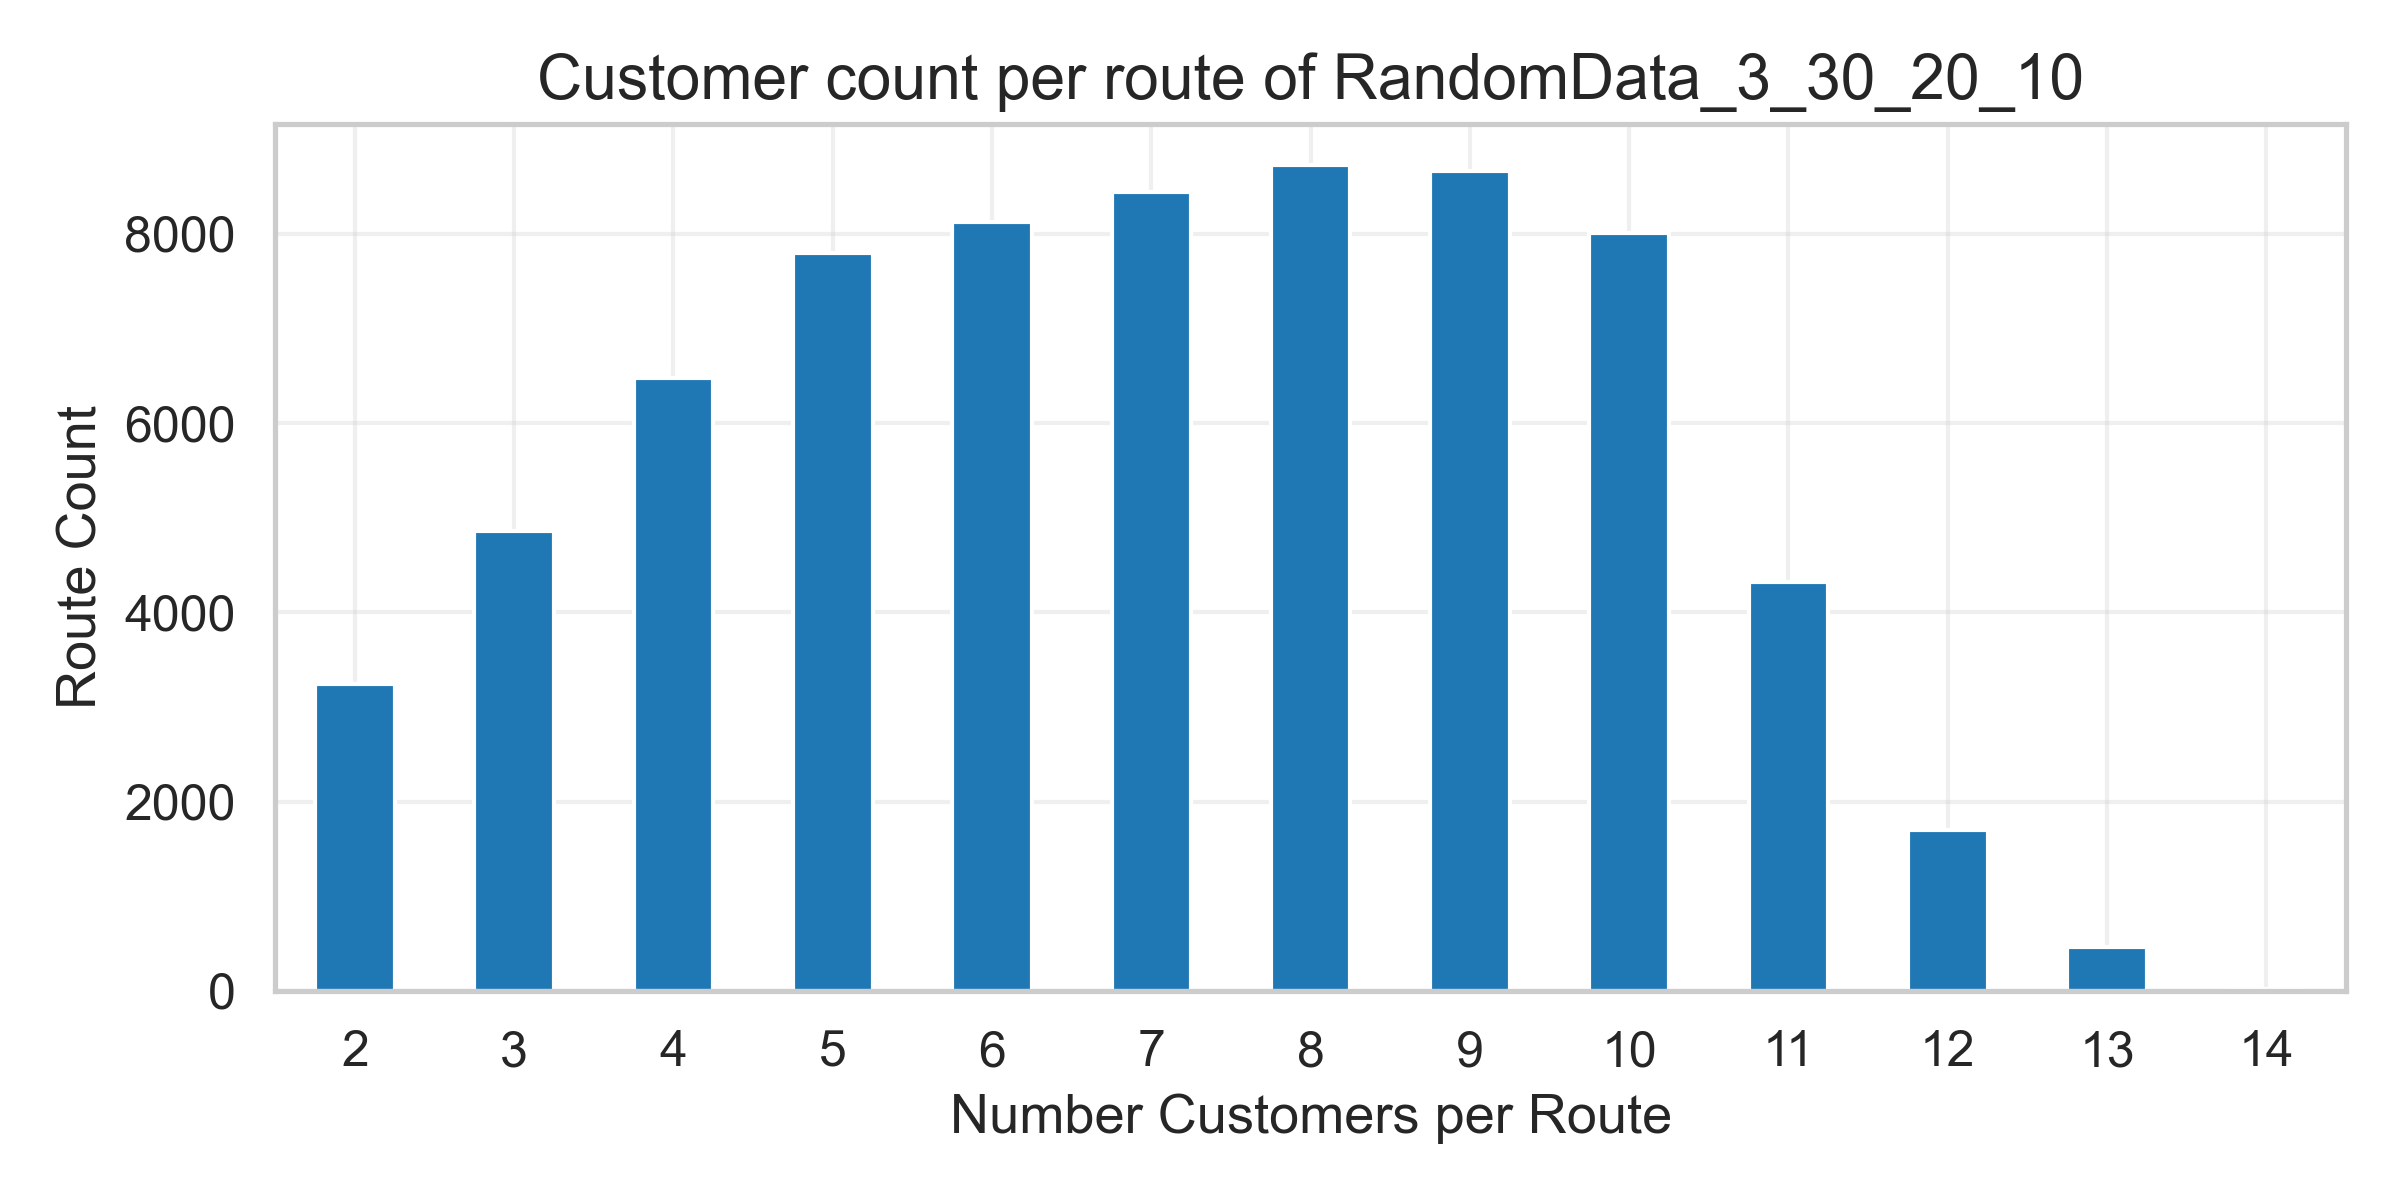
\includegraphics[width=\linewidth]{pictures/dataset_structure/no_cust_plot_RandomData_3_30_20_10.png}
        \caption{RD-3-30-20-10; \\ Threshold $\delta$ = 1.0.}
        \label{fig:ds-c}
    \end{subfigure}
    \caption{Distribution of route length for a randomly generated dataset with different thresholds.
        The red vertical line represents the average number of customers.}
    \label{fig:route-dists_randomdata}
\end{figure}



\subsubsection{Save Retrieval Strategy}

By running the complete B\&C algorithm from \cite{tamke_branch-and-cut_2024}, two train datasets were generated,
one considering the infeasible routes from the \textit{NoSequence} sets and one only the sequences. The prior dataset is
labeled with WS (= with sets). The length of the routes included in the
train dataset are dominated by routes consisting of 2 customers,
as in the beginning of the algorithm all customer combinations are checked to find infeasible customers tuple to
fasten the feasibility loading check in the algorithm afterwards. \footcite[cf.][]{tamke_branch-and-cut_2024}
The results of the branch-and-cut algorithm are summarized in Table~\ref{tab:bc_results_gendreau} in the appendix.
Thhe distribution of the route length is shown in Figure~\ref{fig:customer_count_bc}.
\begin{wrapfigure}{l}{0.5\textwidth}
    \begin{center}
        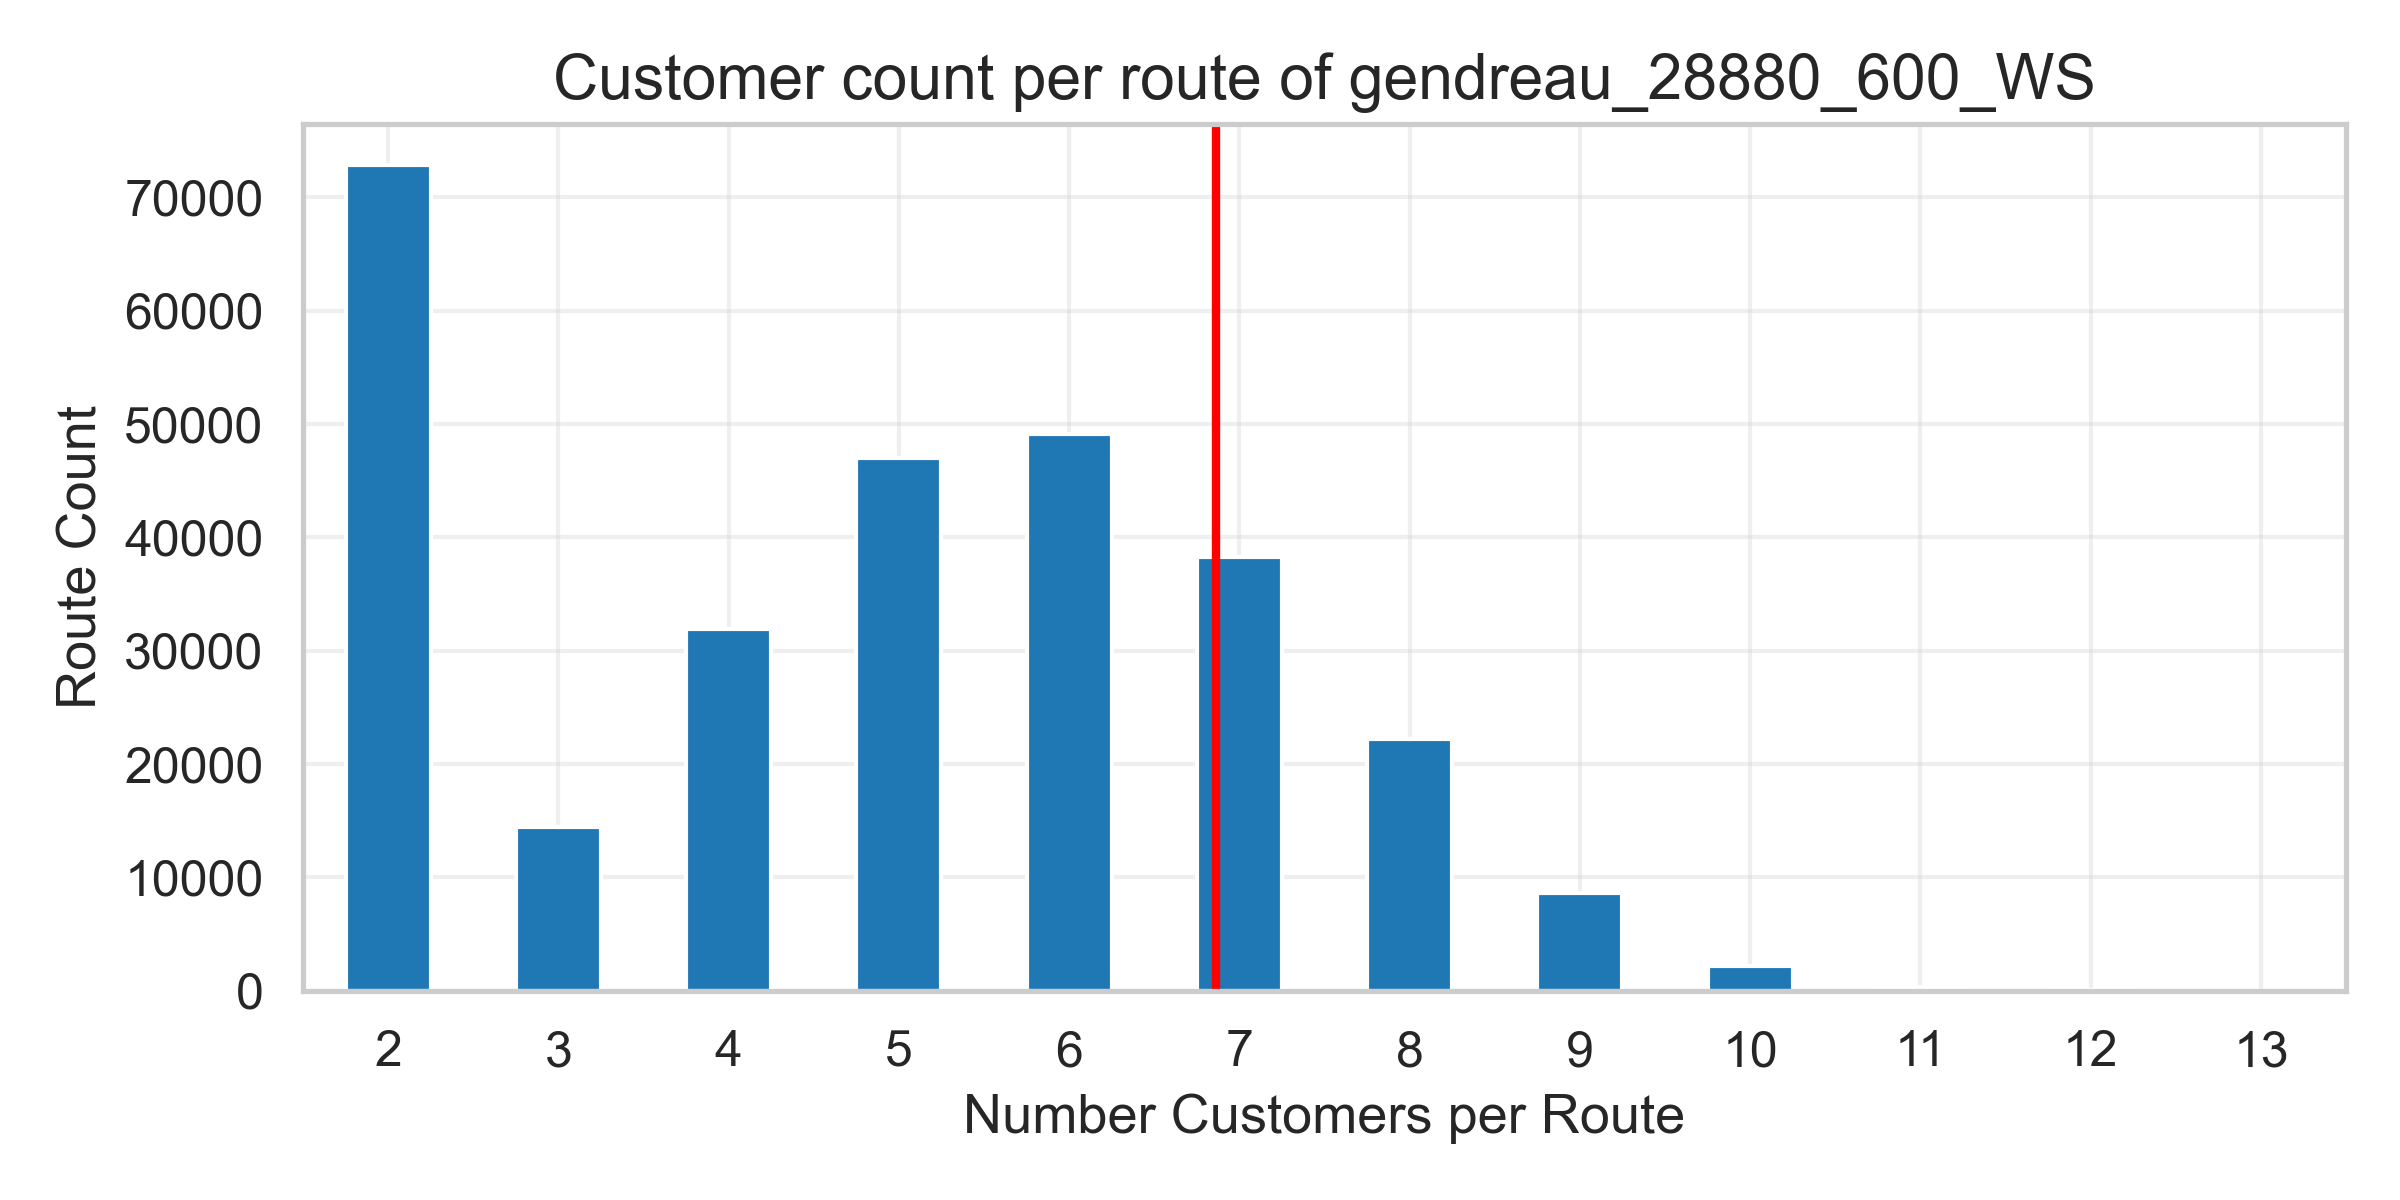
\includegraphics[width = .5\textwidth]{pictures/dataset_structure/no_cust_plot_gendreau_28880_600_WS.png}
        \caption{Customer count per route for dataaset GD-Complete-WS.}
        \label{fig:customer_count_bc}
    \end{center}
\end{wrapfigure}
To reduce the number of routes with two customers, two altenative datasets are constructed for each base dataset to test if the reduction
of number of routes with 2 customers, lead to better model performance results. Therefore it was tested
to shrink all feasible routes with 2 customers with a cosine similarity of $94\%$ (Shrinked) or alternatively drop
all feasible routes with 2 customers (Trimmed).
The resulting datasets have the following characterics, shown in Table~\ref{tab:saved_instances_gendreau}, and it is apparent, that the average relative volume
and mass are higher for the two modified datasets, as short routes were dropped. Additionally the balance between
feasible and infeasible is tilting to more to infeasible tours as only feasible routes with two customers were dropped.
Additonally the WS datasets contain more infeasible routes and are therefore more imbalanced.

\begin{table}[!h]
    \centering
    \small
    \begin{tabular}{l c c c c c c }
        \toprule
        Name           & Sets                 & Routes & Route Len = 2 & Balance   & Rel. Vol & Rel. Mass \\
        \midrule
        GD-Complete-WS & \multirow{3}{*}{Yes} & 286858 & 72832         & 37.6/62.4 & 0.62     & 0.46      \\
        GD-Trimmed-WS  &                      & 216260 & 2234          & 17.2/82.8 & 0.74     & 0.54      \\
        GD-Shrinked-WS &                      & 249564 & 35538         & 28.2/71.8 & 0.68     & 0.50      \\        \midrule
        GD-Complete    & \multirow{3}{*}{No}  & 220825 & 72832         & 48.8/51.2 & 0.55     & 0.43      \\
        GD-Trimmed     &                      & 150227 & 2234          & 24.7/75.3 & 0.69     & 0.53      \\
        GD-Shrinked    &                      & 183531 & 35538         & 38.4/61.6 & 0.61     & 0.48      \\
        \bottomrule
    \end{tabular}
    \caption[Save strategy train datsets from \gendreauDataSet.]{Save strategy train datsets from \gendreauDataSet.}
    \label{tab:saved_instances_gendreau}
\end{table}

\subsubsection{Differences between Random and save strategy datasets}

As the creation method differs significantly between the random and the save strategy, differences are laid out in
the following paragraph. The branch-and-cut algorithm does not follow any strict route generation procedure, but to
find the optimal solution for each instance. The complexity to solve these is aligned with the number of routes found.
Therefore only few routes from simple instances, belonging to $\mathcal{H}$, are considered in the save strategy dataset
in comparison to the random datasets. This difference is visualized in the following Figure~\ref{fig:comparison_noroutes_perInstancce}
visualizing the number of routes and the labels per instance of \gendreauDataSetText considered in each training dataset.

\begin{figure}[ht]
    \centering
    \begin{subfigure}[t]{.5\textwidth}
        \centering
        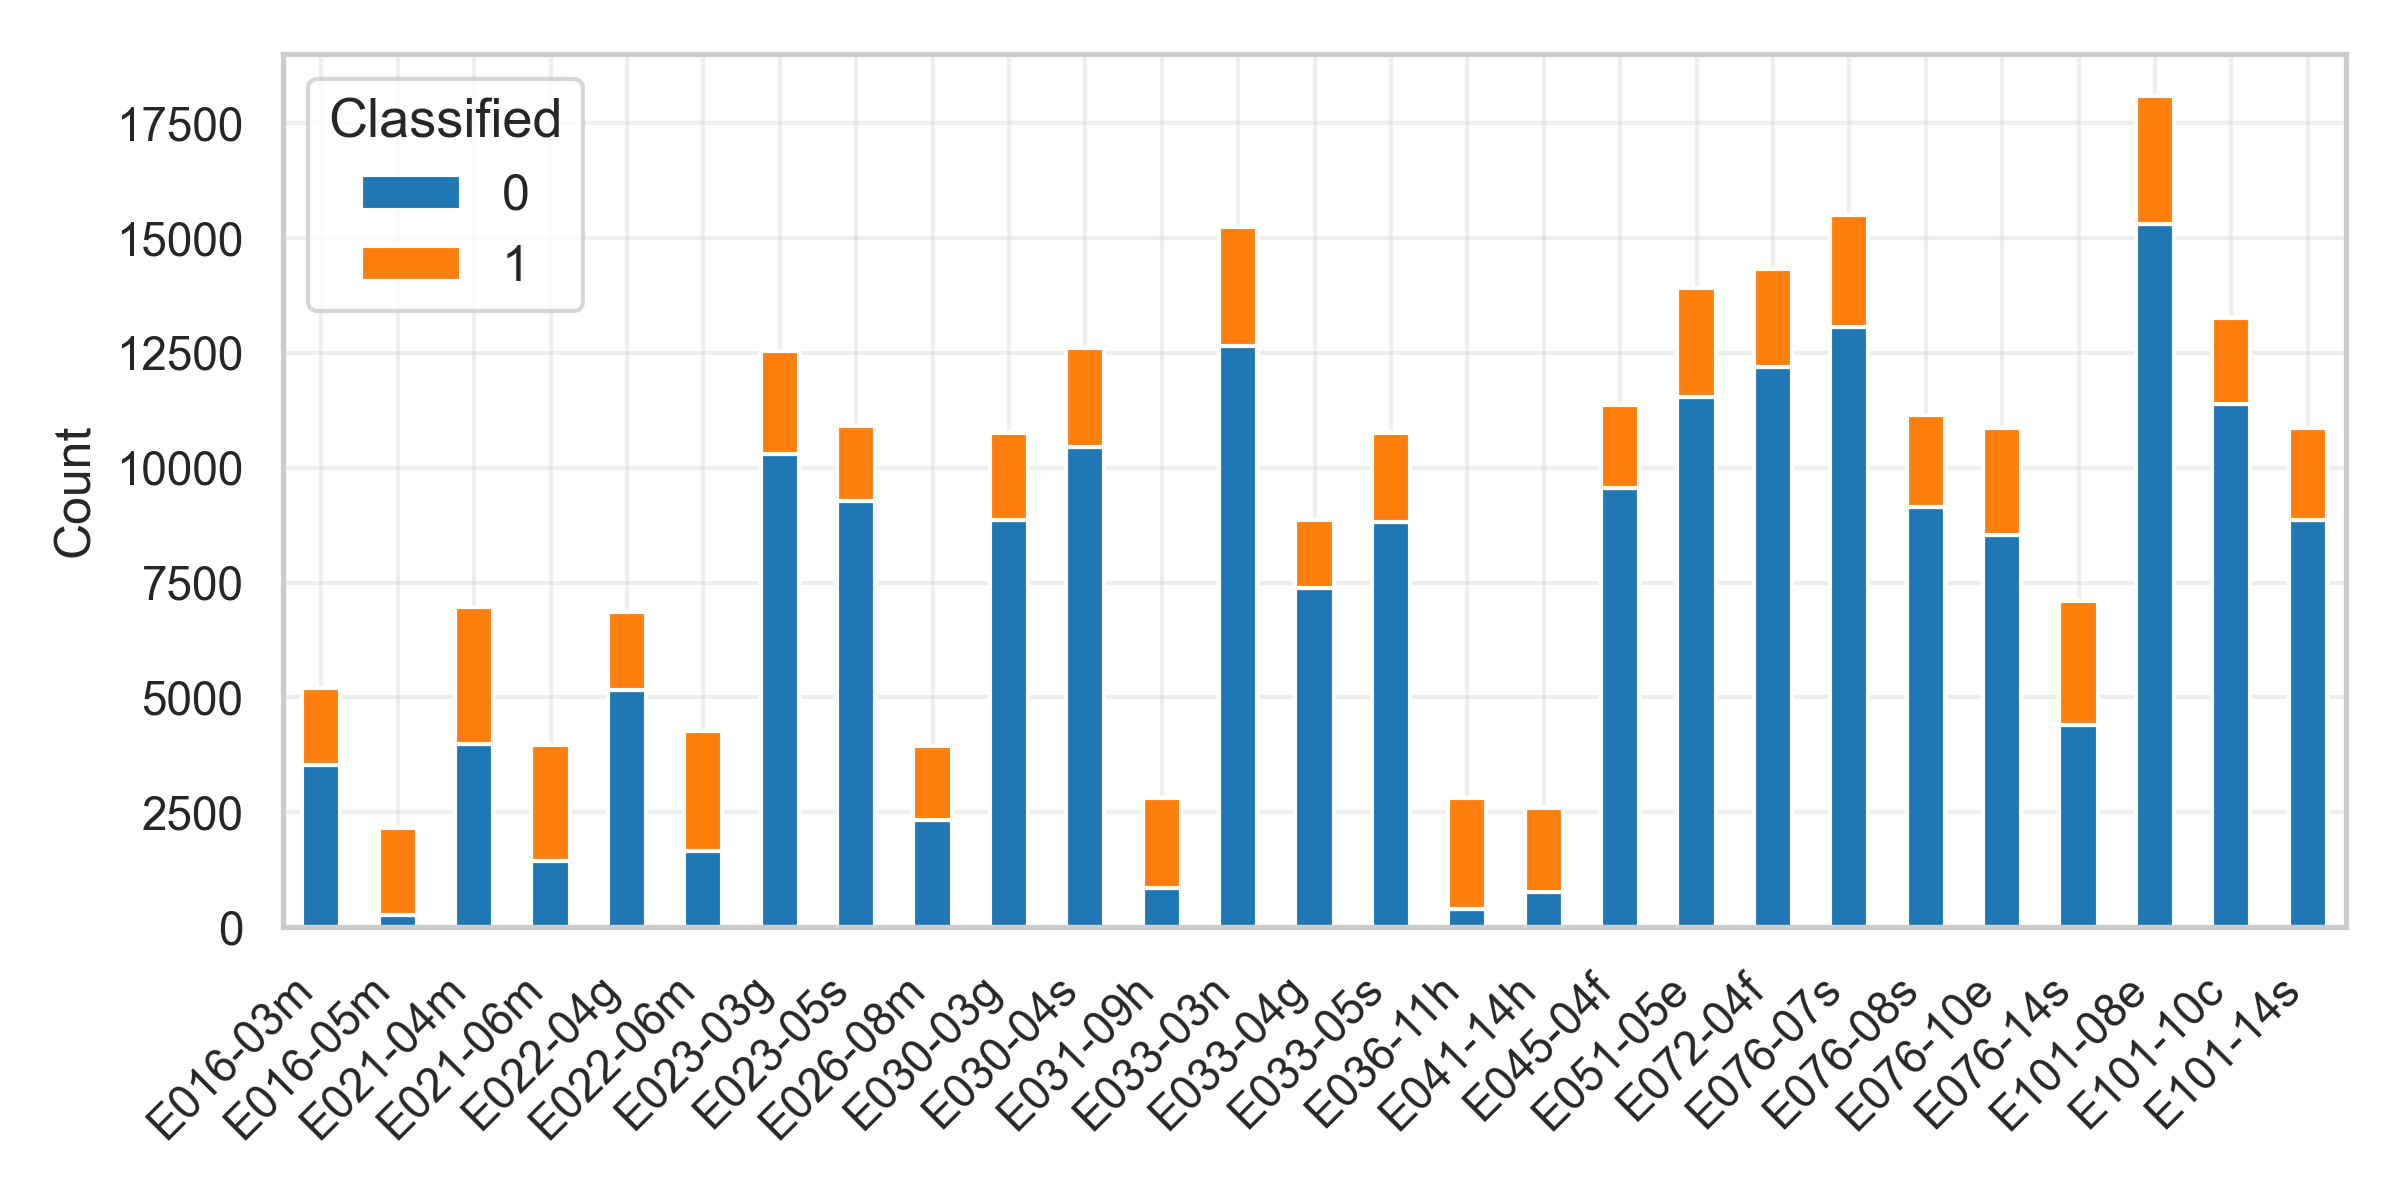
\includegraphics[width=\linewidth]{pictures/dataset_structure/distribution_plot_RandomData_5_40_40_10.png}
        \caption{Random dataset RD-3-30-20-8.}
    \end{subfigure}%
    \begin{subfigure}[t]{.5\textwidth}
        \centering
        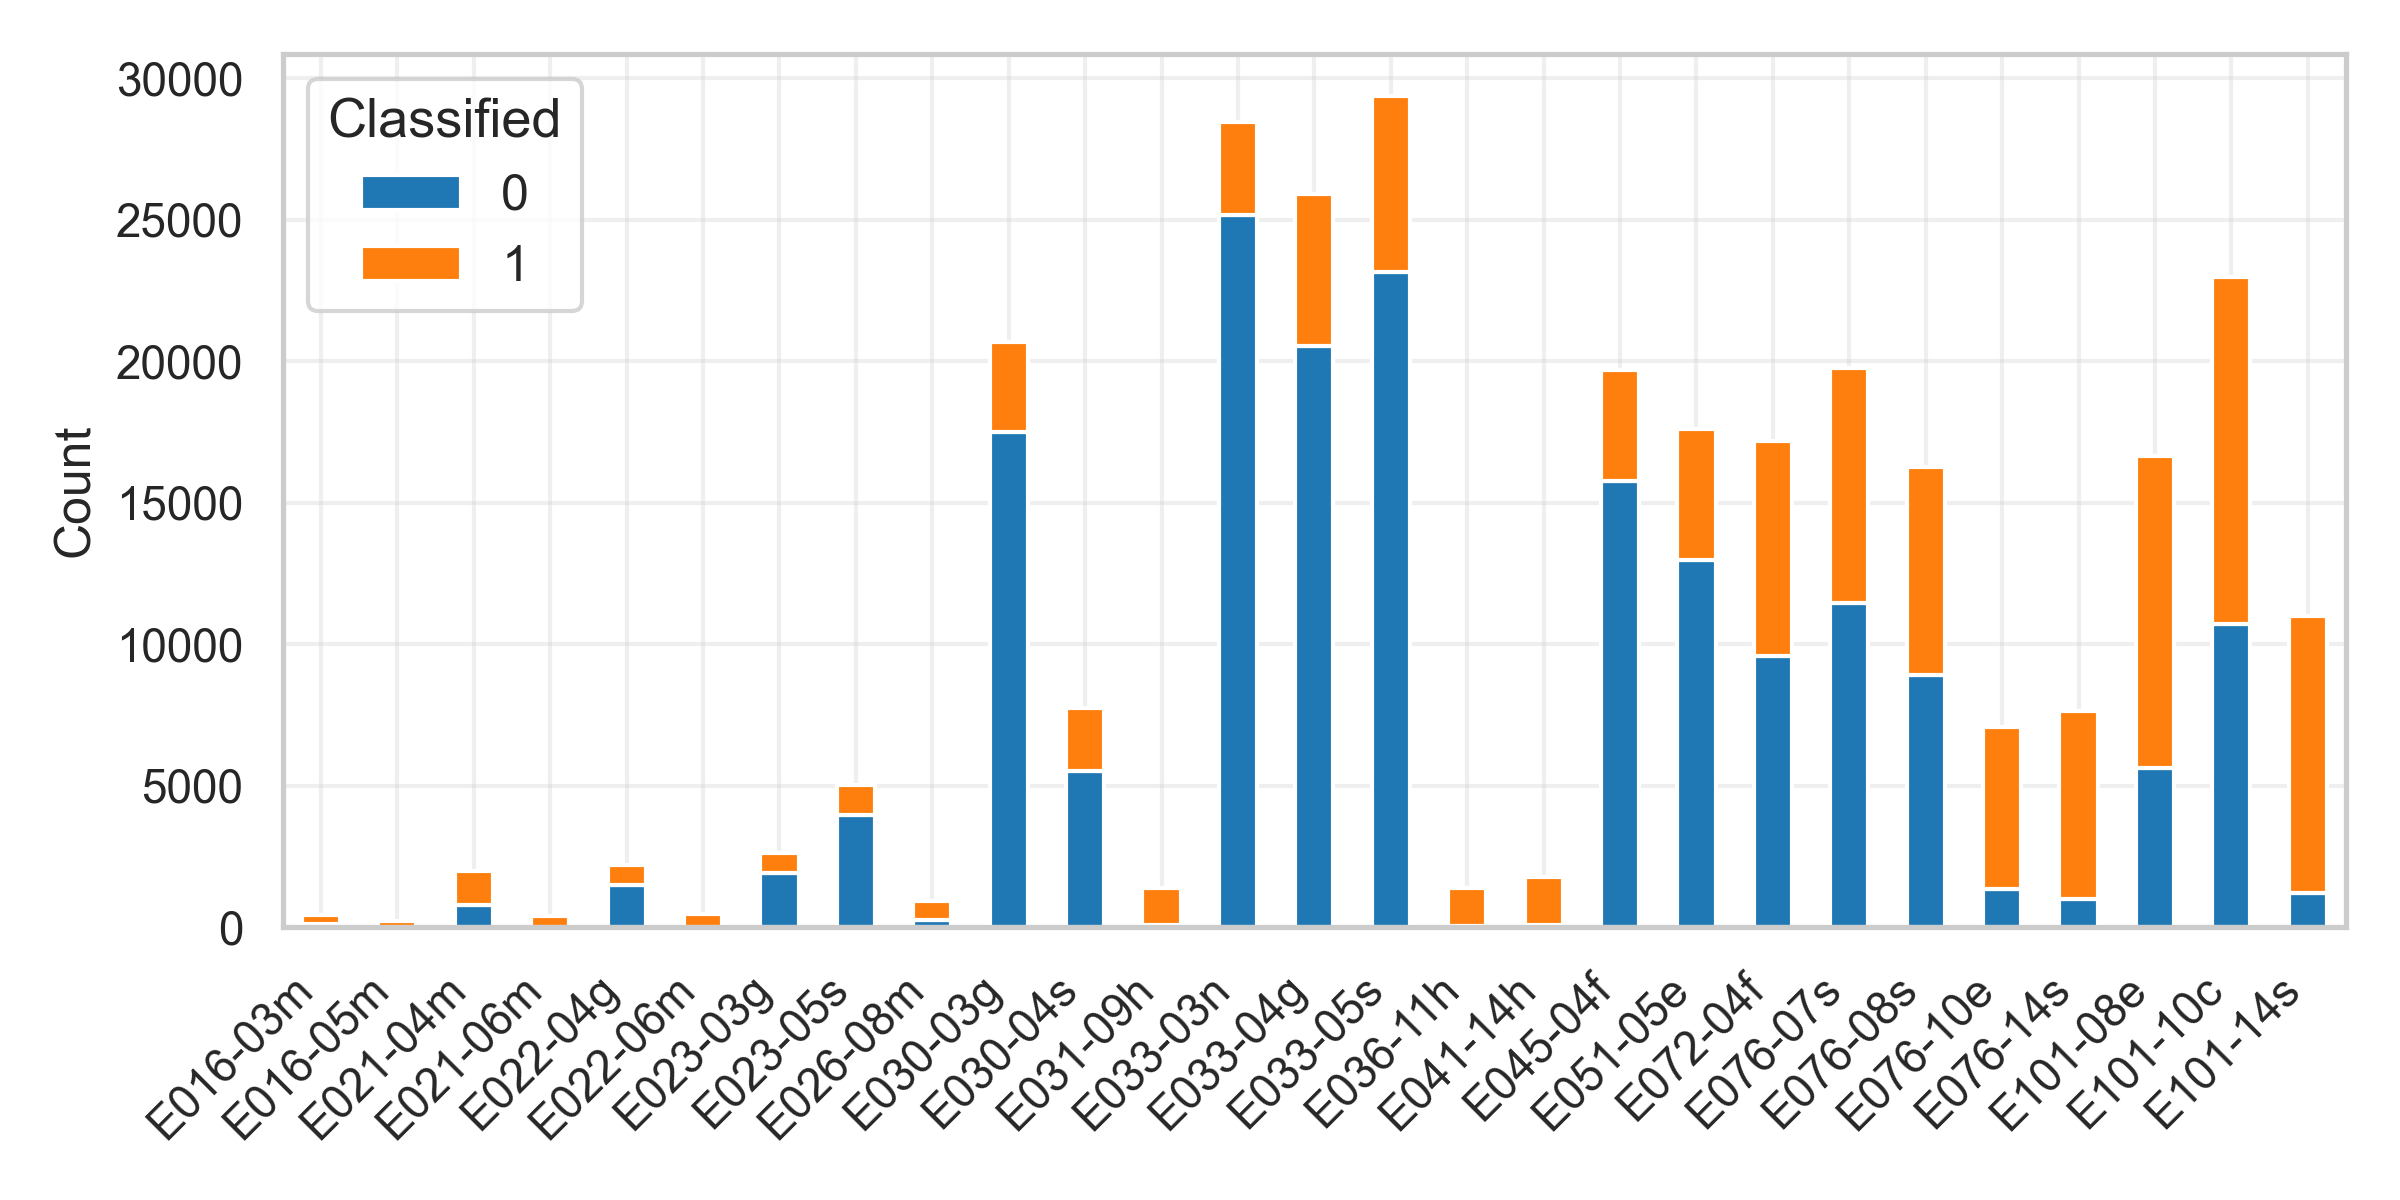
\includegraphics[width=\linewidth]{pictures/dataset_structure/distribution_plot_gendreau_28880_600_WS.png}
        \caption{Save strategy dataset Complete-WS.}
    \end{subfigure}
    \caption{Distribution of routes considered per instance for two exemplary datasets of random and save strategy.}
    \label{fig:comparison_noroutes_perInstancce}
\end{figure}

\subsection{Feature Filter Results}
\label{sec:feature_filter_results}

The filter Algorithm~\ref{alg:filter_algorithm} was applied for each of the following minimum importance thresholds
$\epsilon =[0.1,0.2.3,0.4]$ and barriers $\mathcal{B}=[0.5,0.75]$ . Furthermore, the pearson correlation thresholds $\Phi$ = [0.8, 0.85, 0.9] and
all 27 datasets, forming $\mathcal{D}$, presented in the previous subsection were considered. Figure~\ref{fig:feature_filter_parameters}
in the appendix shows, how each set is constructed visualizing
different thresholds $\epsilon$ and the influence of the barrier $\mathcal{B}$. It needs to be noted, that
the thresholds below 20\% were considered, but these had no impact on the final subset. The list of the
features which will be dropped are shown in Table~\ref{tab:feature_dropsets}. The following Table~\ref{tab:drop_set_presentation_shortened}
presents the names of the drop sets as well as the number of features, which will be dropped.
Additionally, one empty dropset (DS-0-0) was added, to analyse the impact of the dropsets.
\begin{table}[ht]
    \centering
    \small
    \begin{tabular}{l c c c c c c c}
        \toprule
        Dropset Name          & DS-50-2 & DS-50-3 & DS-50-4 & DS-75-2 & DS-75-3 & DS-75-4 & DS-0-0 \\
        \midrule
        Barrier $\mathcal{B}$ & 0.5     & 0.5     & 0.5     & 0.75    & 0.75    & 0.75    & -      \\
        Threshold $\epsilon$  & 0.2     & 0.3     & 0.4     & 0.2     & 0.3     & 0.4     & -      \\
        Number Features       & 10      & 18      & 38      & 7       & 18      & 32      & 0      \\
        \bottomrule
    \end{tabular}
    \caption{Presentation of the considered drop sets for the feature selection.}
    \label{tab:drop_set_presentation_shortened}
\end{table}

For each dropset each dataset was trained for each model type and was used to predict the true labels of
every other dataset to select the best fitting dropset. The used hyperparameters for each model can be seen in
Table~\ref{tab:hyperparams_feature_selection} in the appendix. For the following analysis of the results, it
needs to be noted, that all results predicting from one save strategy dataset to another was excluded,
as every dataset is a subset of each other (see Table~\ref{tab:saved_instances_gendreau}).
The following Figure~\ref{fig:mcc_filter_results} shows the performance of boxplots for the \gls{MCC} for all drop sets
and the three different model types introduced in Section~\ref{sec:modelselection}.

\begin{figure}[ht]
    \centering
    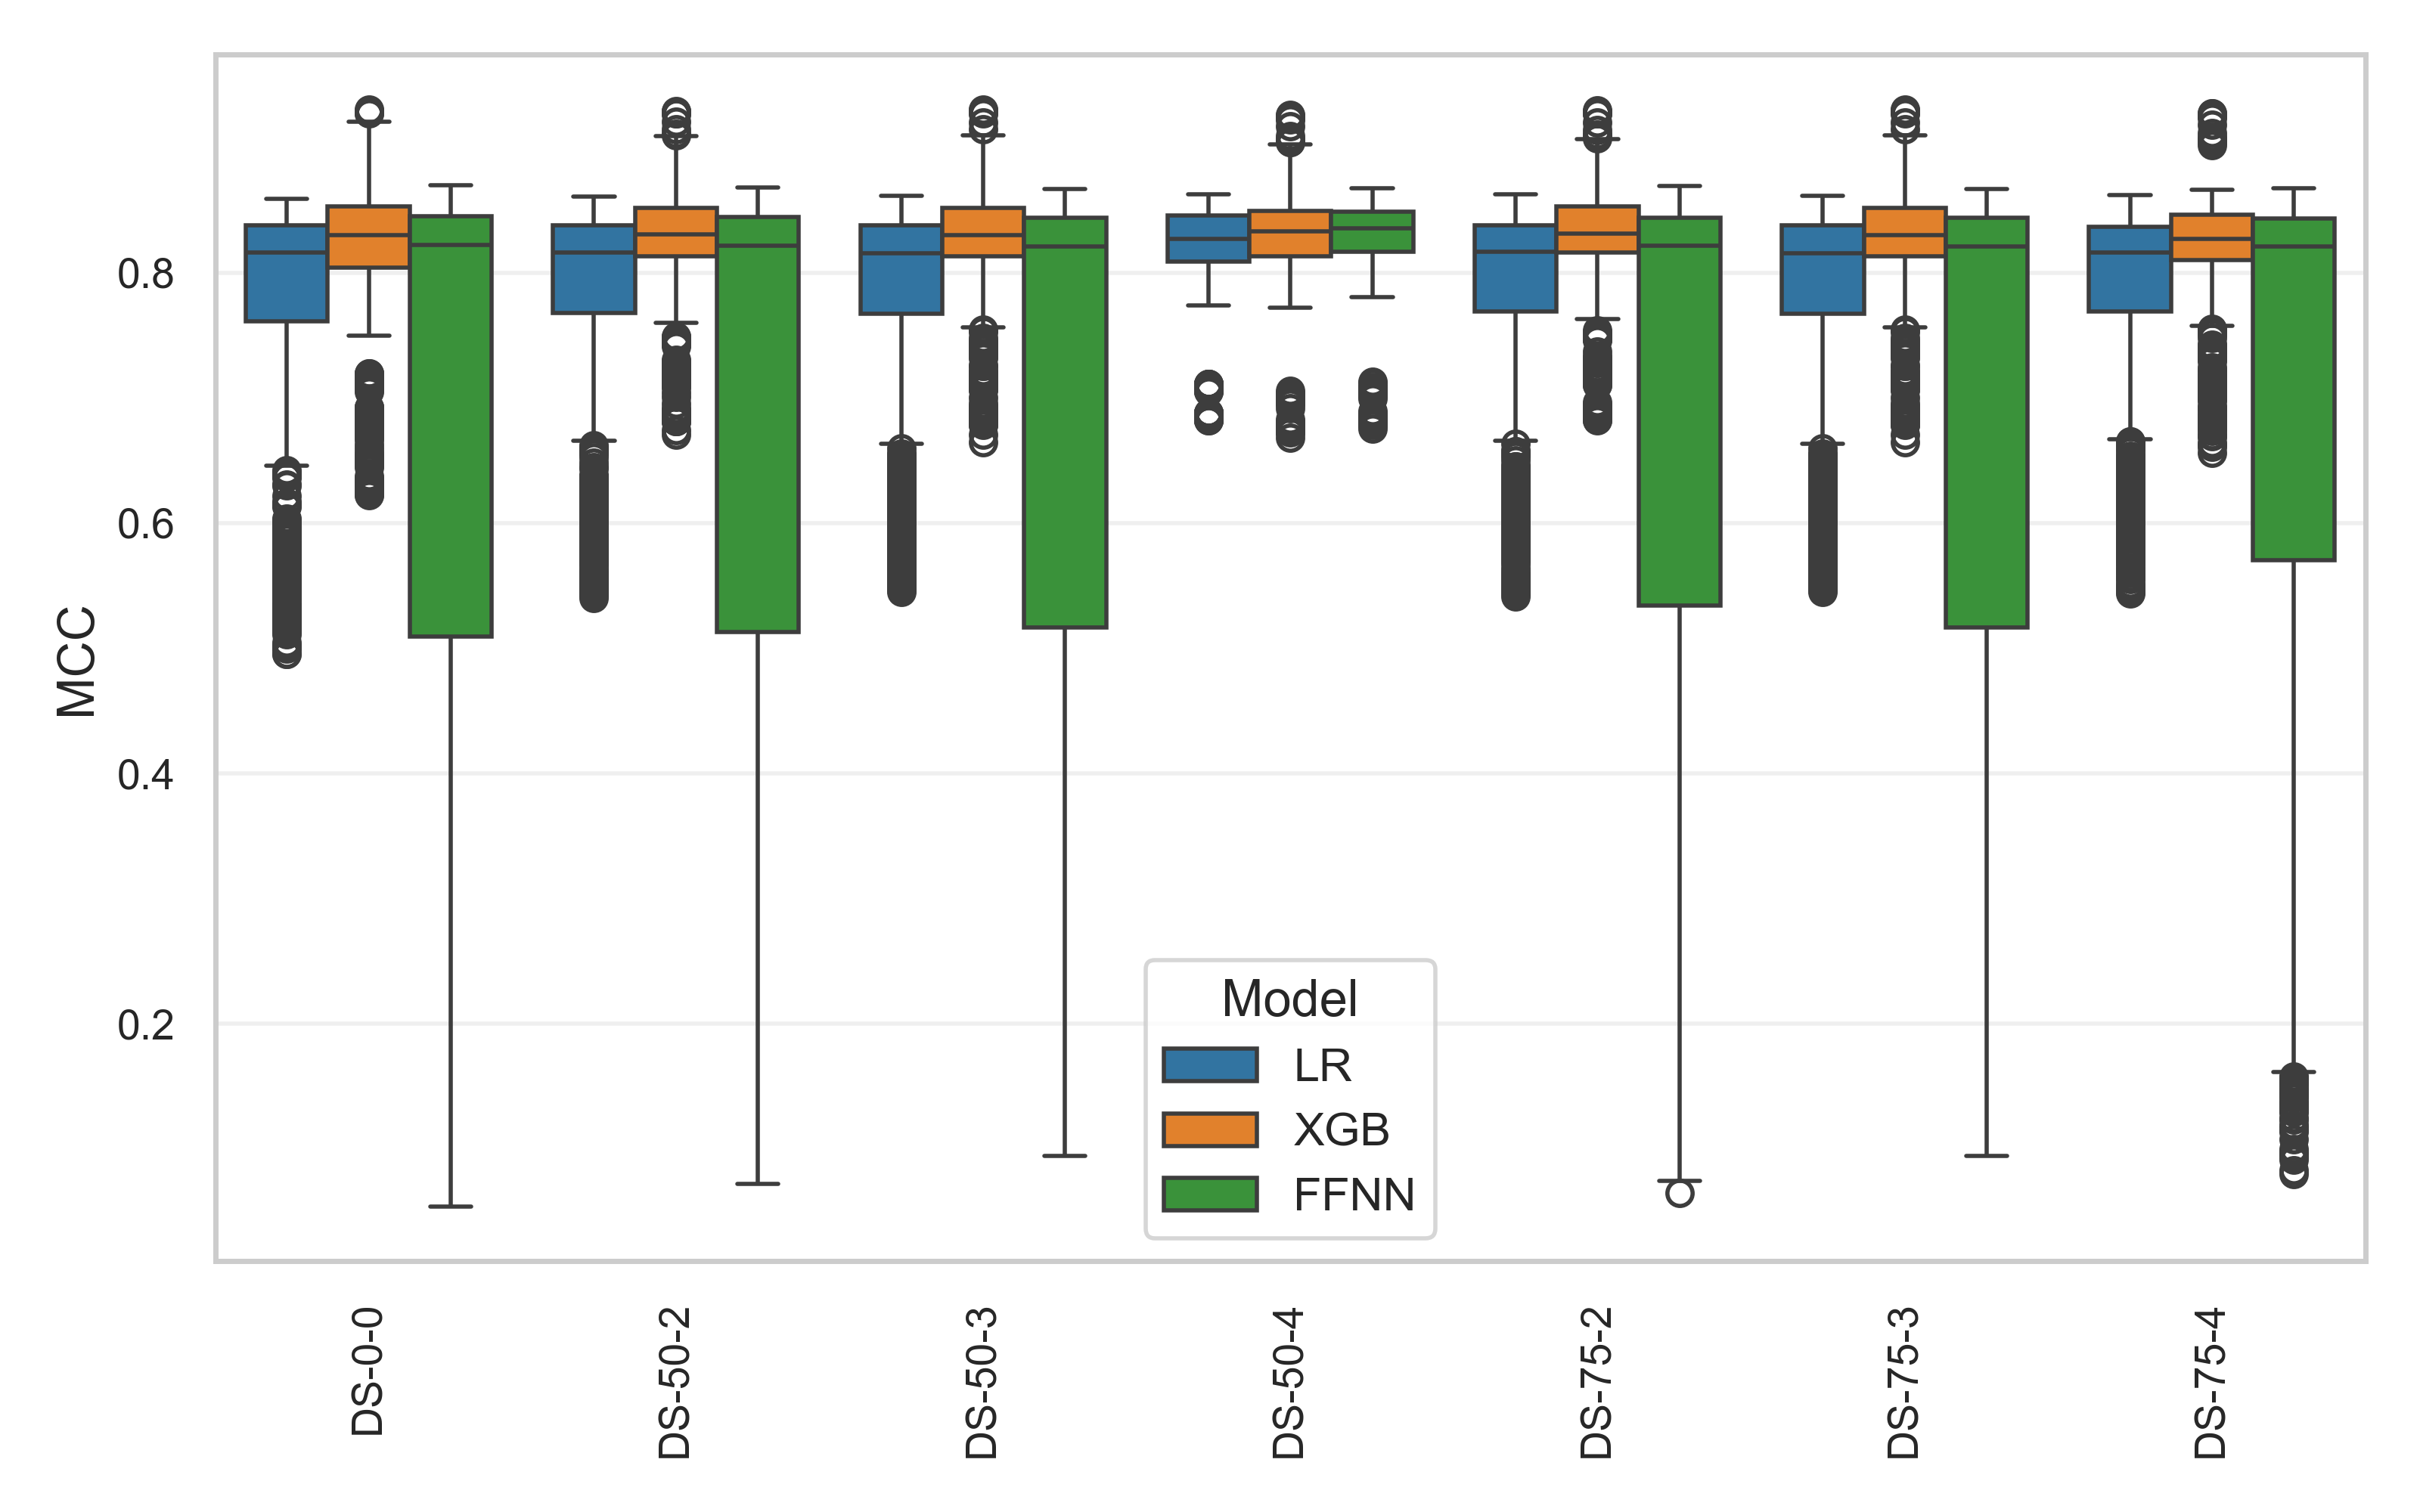
\includegraphics[width = .95\textwidth]{pictures/feature_filter/all_data_exceptSubsets_box_plot.png}
    \caption{Box plots of MCC performance of different feature drop sets.}
    \label{fig:mcc_filter_results}
\end{figure}
Two things are apparent in the boxplot, first the model performance for the \gls{FFNN} has the greatest spread performance-wise and
XGB the smallest. Second, the results for dropset DS-50-4 are the most constant having very similar results. For both, the \gls{LR} and
the \gls{FFNN} the spread is greater as for the XGB model caused by the need to scale the data before the prediction is done on all datasets.
The scaling depends on the train dataset the model is initially trained on, if the structure, the mean and the standard deviation is
different \footnote{Compare Table~\ref{tab:saved_instances_gendreau} and Table~\ref{tab:created_instances_xyz_gendreau} for the created datasets.}
the scaled feature values on the predicting datasets, will have other ranges than the initially train dataset, causing the model to perform worse.
The \gls{FFNN} is here more "sensitive" than the \gls{LR} model, due to the amplified effect of the hidden layers of the model. The dropset
DS-50-4 removes 38 of 48 intital features, reducing the complexity and the possibility to "mis-scale" data to a minimum, while preserving
the same model predicting performance as can be seen in the comparison of the boxplots. The results for all performance metrics is shown in
the following Table~\ref{tab:featurePerformance_Alldata}.

\begin{table}[ht]
    \centering
    \small
    \begin{tabular}{lrrrrrrr}
        \toprule
        DropSet  & DS-0-0 & DS-50-2 & DS-50-3 & DS-50-4       & DS-75-2 & DS-75-3 & DS-75-4 \\
        \midrule
        MCC      & 0.75   & 0.76    & 0.76    & \textbf{0.82} & 0.76    & 0.76    & 0.76    \\
        F1-Score & 0.81   & 0.82    & 0.82    & \textbf{0.88} & 0.82    & 0.82    & 0.82    \\
        Accuracy & 0.89   & 0.89    & 0.89    & \textbf{0.93} & 0.89    & 0.89    & 0.89    \\
        AUROC    & 0.96   & 0.96    & 0.96    & \textbf{0.98} & 0.95    & 0.96    & 0.96    \\
        \bottomrule
    \end{tabular}
    \caption[Mean performance metrics on various different drop set excluding the performance from save strategy datasets to save strategy datasets.]
    {Mean performance metrics on various different drop set excluding the performance from save strategy datasets to save strategy datasets.
        Bold font shows the best results for each performance score.}
    \label{tab:featurePerformance_Alldata}
\end{table}

The final features considered for predicting the loading feasibility are the following:
\begin{table}[ht]
    \centering
    \def\arraystretch{1.5}
    \begin{tabular}{l l l l }
        $\bullet$ Rel Volume     & $\bullet$ Fragile Sequence   & $\bullet$ width-W-mean & $\bullet$ height-H-std    \\
        $\bullet$ length-L-std   & $\bullet$Weight Distribution & $\bullet$ width-W-std  & $\bullet$ height-area-min \\
        $\bullet$ area-AREA-mean & $\bullet$ area-AREA-max      &                        &                           \\
    \end{tabular}
\end{table}

In the Section~\ref{app:sec:further_feature_filter} in the appendix more feature filter insights are presented, but the
results stay the same, that drop set DS-50-4 has the overall best results and that the performance of models with the need
to scale the features lack performance, considering many different datasets. The next section is about choosing the
datasets further used as classifiers in the final algorithm.

\subsection{Selection of dataset}
\label{sec:dataset_selection}

The results obtained from the feature filter perfromance analyses descirbed in the previous section, can be used to analyze and select
the best performing datasets from each retrieval strategy, when the results are filtered for drop set DS-50-4.
The folllowing Figure~\ref{fig:dataset_performance_group_subgroup} displays the \gls{MCC} performance based on which base dataset is chosen (Group)
and which subgroup of datasets are predicted, either random or save strategy datasets. As described in the previous section, only the
performance on the base dataset is considered for the save strategy datasets as the datasets are subsets from each other.
\begin{figure}[ht]
    \centering
    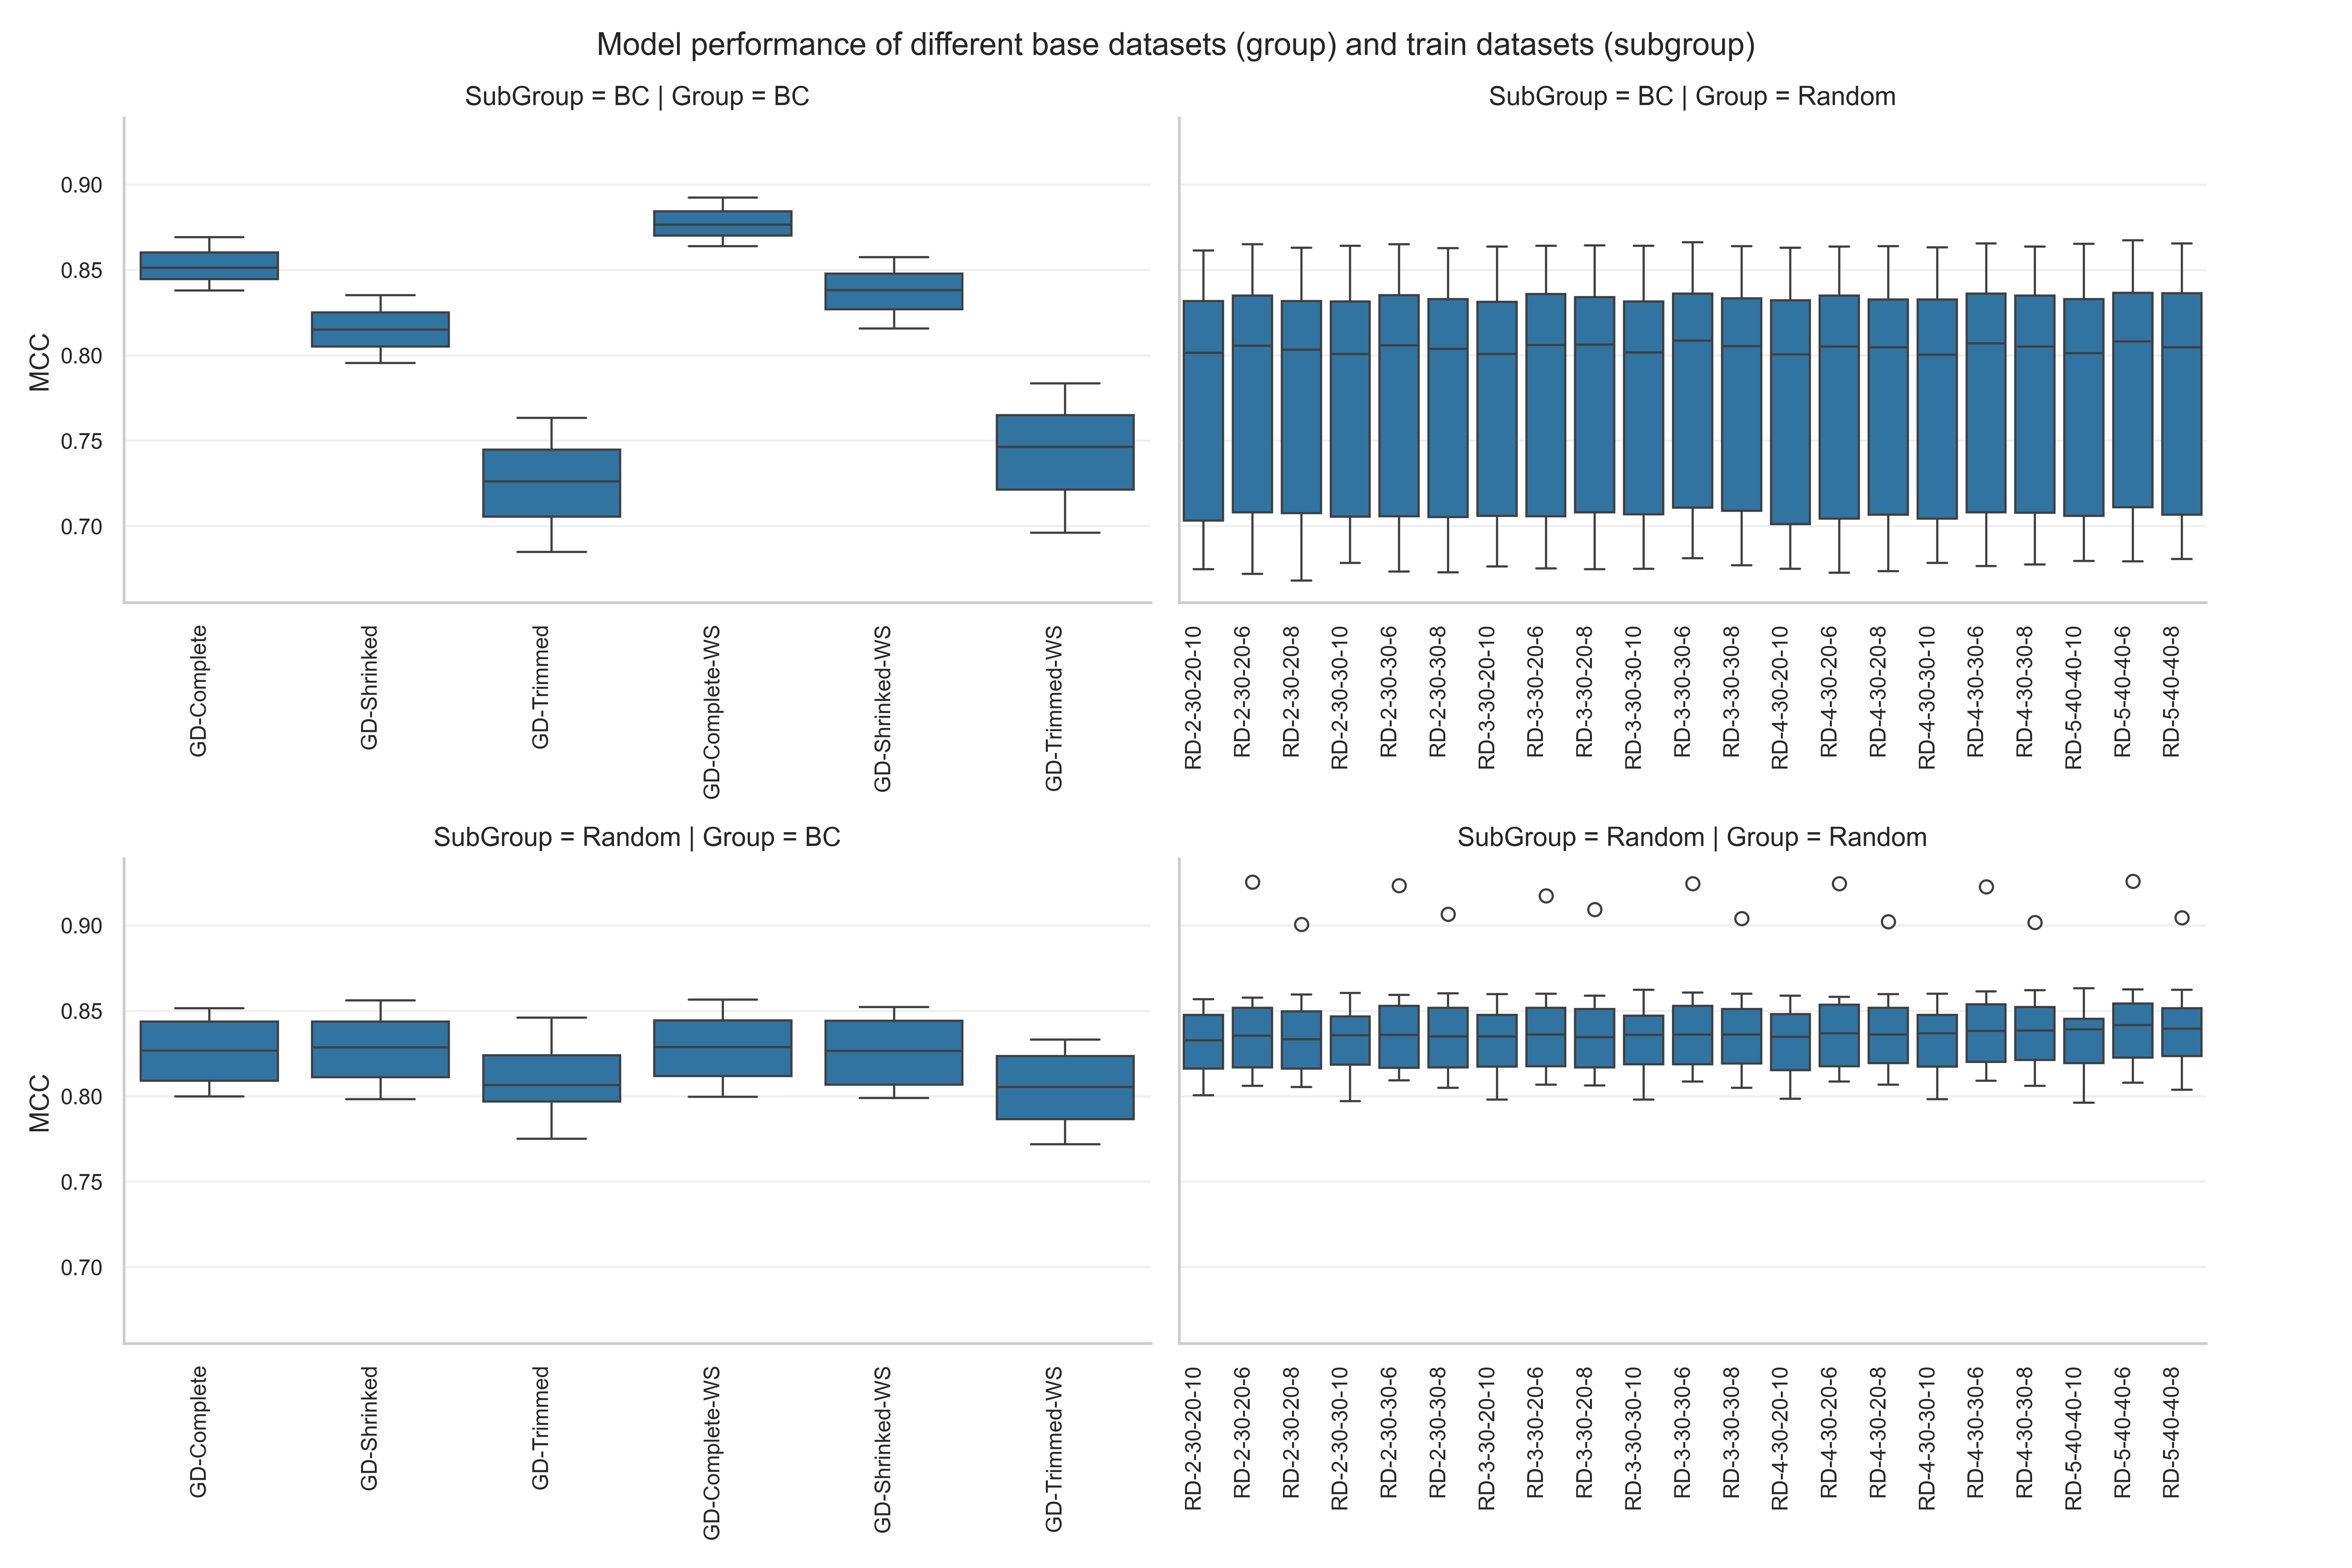
\includegraphics[width =\textwidth]{pictures/feature_filter/group_subgroup_results.png}
    \caption{Box plots of MCC performance of different feature drop sets.}
    \label{fig:dataset_performance_group_subgroup}
\end{figure}

The first subplot Group = SubGroup = BC, displays therefore only the performance on the base train dataset for every respected model type (\gls{LR}, XGB and \gls{FFNN}).
This subset is the only one with significant differences in performances and the complete datasets outperform the other. When the subgroup
are random datasets, the performance of shrinked and complete is similar. Only the trimmed datasets can be left out for consideration, as
the prediction capability is restricted for small tours as only infeasible routes with two customers are respected. The results for the random
dataset is harder to intepret as the median performance is almost constant for all datasets. When group and subgroup are random datasets, it can
be observed, that the median performance is slightly better for smaller values of $\delta$ in the same group of ($\alpha$, $\beta$, $\gamma$).
To avoid choosing datasets arbitrarily, an additional validation dataset was constructed by saving the routes found during the base \gls{ILS}
algorithm only using the \gls{CP} solver for the feasibility checks. Each instance from \gendreauDataSetText is run 5 times with different times
with an extended timelimit of 15 min to find many different route candidates. The \gls{ILS} parameters for this run are presented in the next section
in Table~\ref{tab:parameters_final_noclassifier}.

\begin{table}[!h]
    \centering
    \small
    \begin{tabular}{l c c c c c }
        \toprule
        Name          & Routes & Route Len = 2 & Balance   & Rel. Vol & Rel. Mass \\
        \midrule
        Validation DS & 427048 & 8605          & 47.0/53.0 & 0.61     & 0.60      \\
        \bottomrule
    \end{tabular}
    \caption{Validation dataset constructed from \gendreauDataSet with ILS.}
    \label{tab:validation_dataset_gendreau}
\end{table}

\begin{figure}[ht]
    \centering
    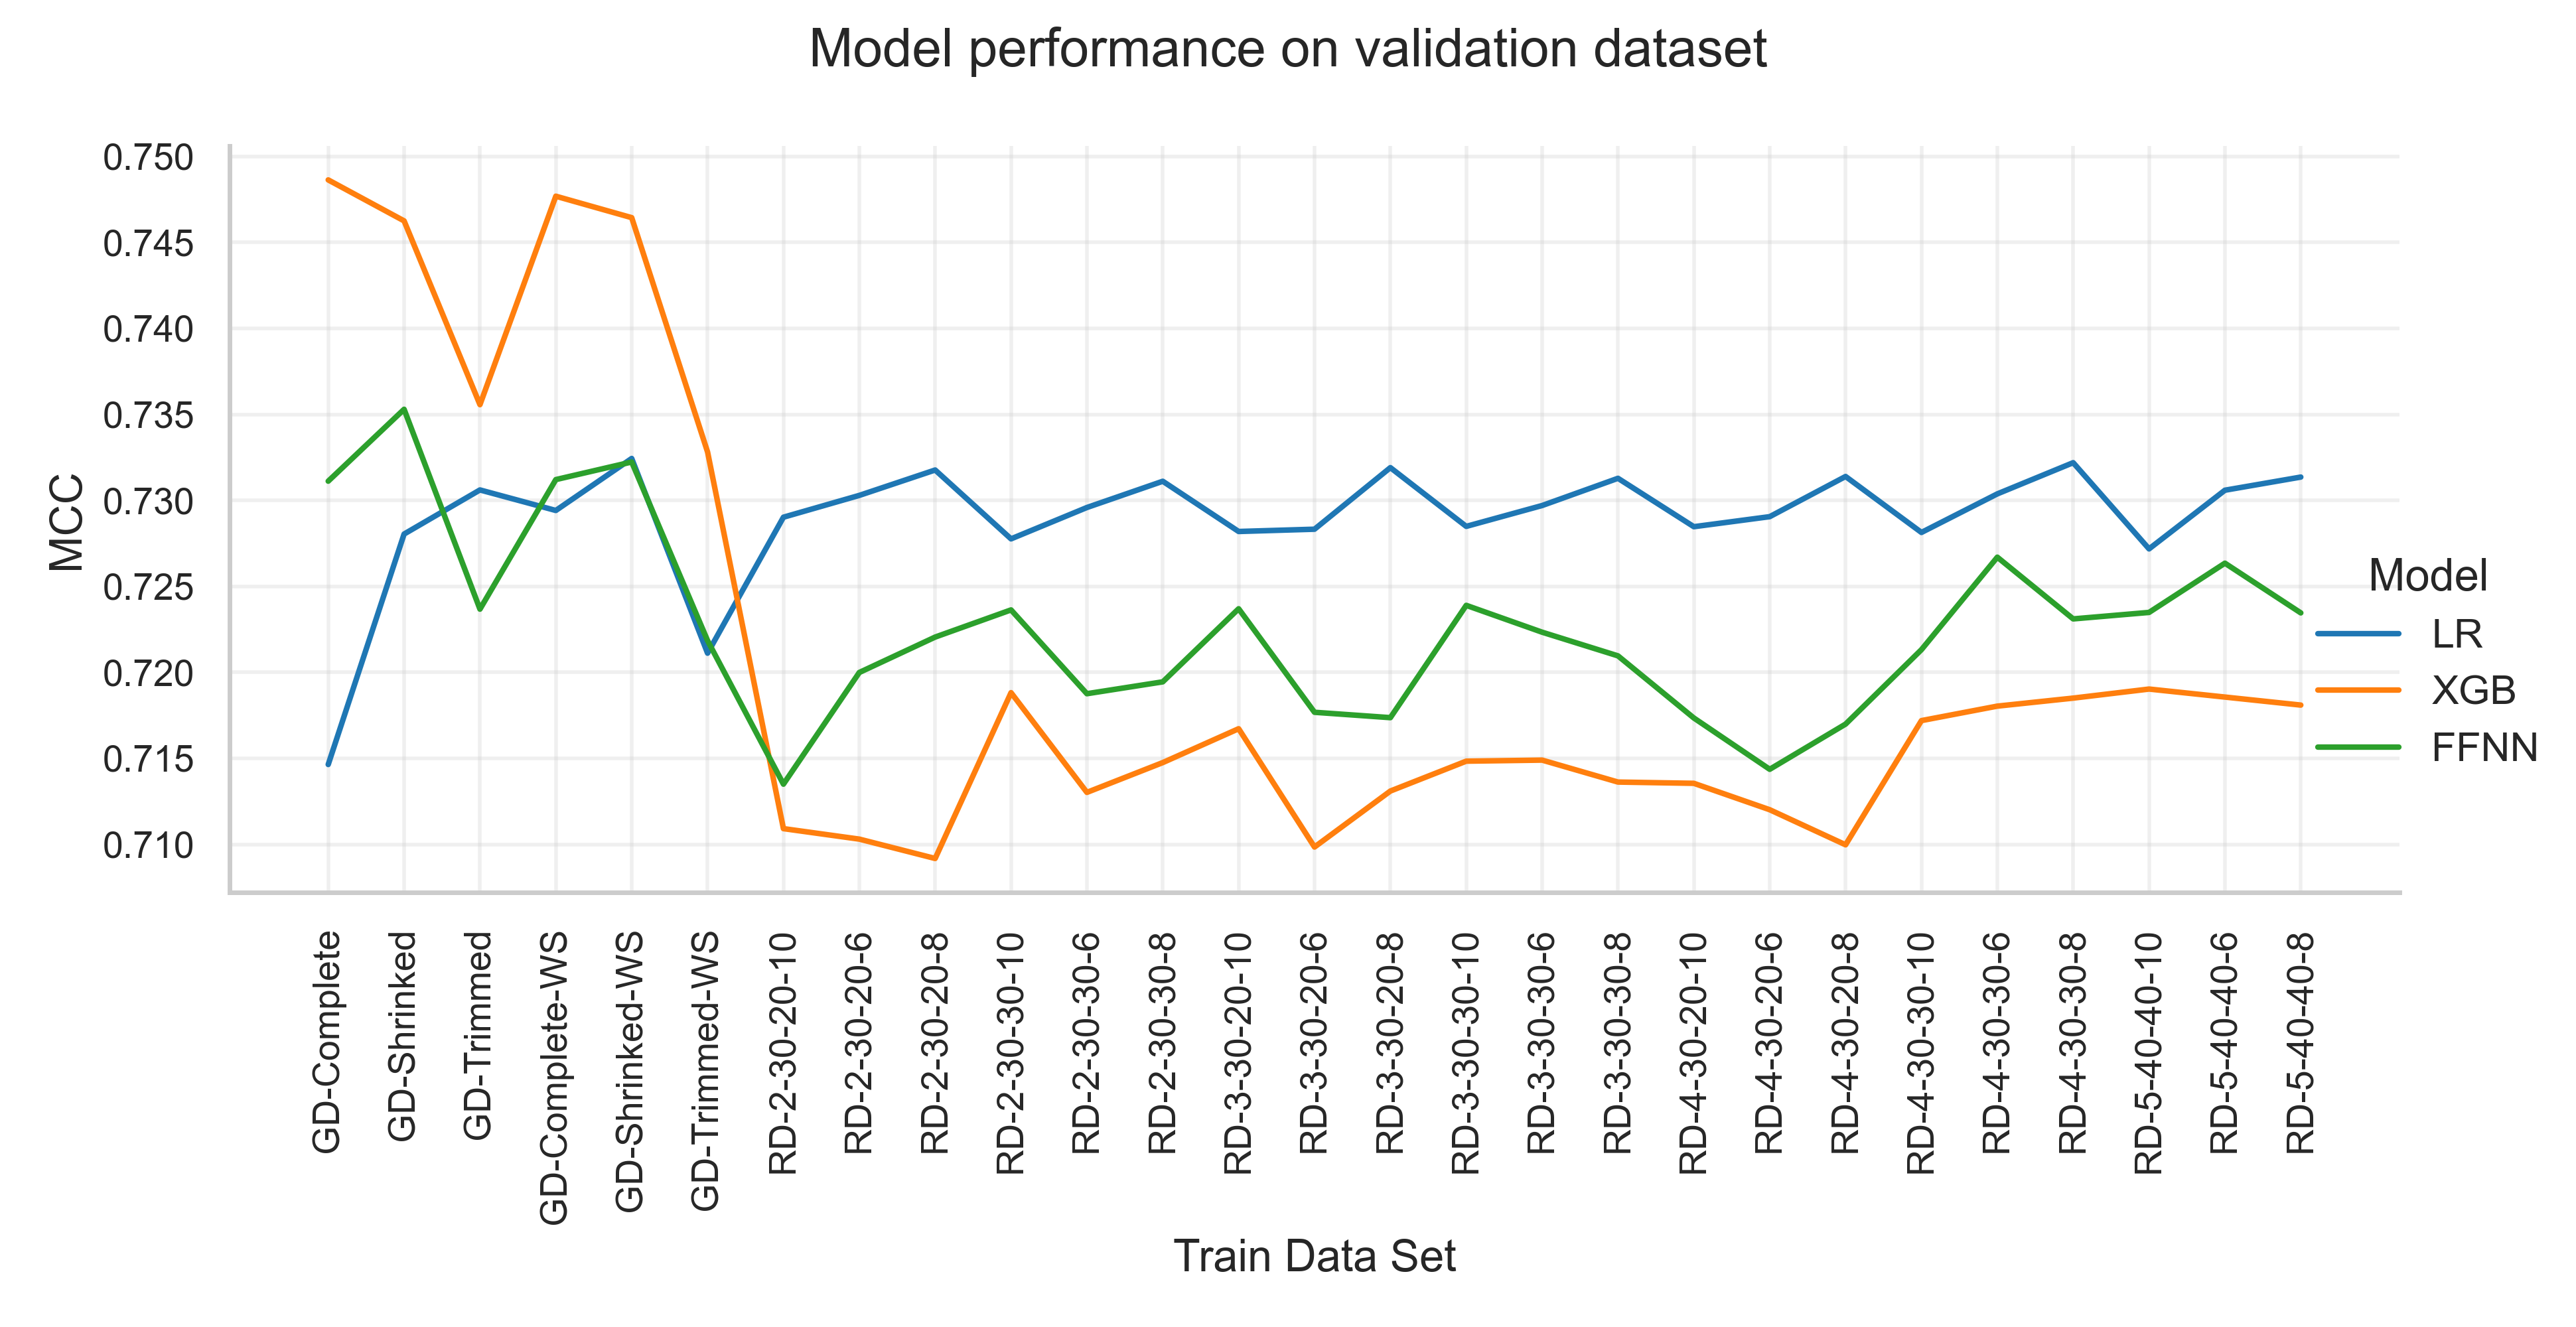
\includegraphics[width =\textwidth]{pictures/feature_filter/validation_line_plot.png}
    \caption{Obtained MCC from validation dataset based on different train datasets and model types.}
    \label{fig:validation_performance_line_plot}
\end{figure}


All the concrete results for every performance metric is depicted in Table~\ref{tab:featurePerformance_validationDataset}.

Chosen Datasets:

\begin{table}[ht]
    \centering
    \setlength{\tabcolsep}{0.75em}
    \def\arraystretch{1.5}
    \begin{tabular}{l|ll}
        Save Strategy   & GD-Shrinked  & GD-Shrinked-WS \\\hline
        Random Strategy & RD-4-30-30-6 & RD-4-30-30-8   \\
    \end{tabular}
\end{table}

\section{Parameter Study}
\label{sec:parameter_study}

The parameter study is divided in four subsections following the variants of the algorithm
presented in Section~\ref{sec:FeasibilityCheck}. This study follows a hierarchical procedure
tuning the parameters, introduced for each variant, sequentially. The following subset of 13
instances from \gendreauDataSetText is used:


\begin{table}[ht]
    \centering
    \setlength{\tabcolsep}{0.75em}
    \def\arraystretch{1.5}
    \begin{tabular}{lllllll}
        E016-03m & E022-04g & E023-03g & E023-05s & E030-03g & E033-04g & E033-05s \\
        E051-05e & E072-04f & E076-07s & E076-14s & E101-10c & E101-14s &          \\
    \end{tabular}
\end{table}

The division followed the following approach, first all instances were omitted, which found
the optimal solution in a short time (see \cite{tamke_branch-and-cut_2024}\footcite[cf.][p.26]{tamke_branch-and-cut_2024}).
Second, similar instances of size and complexity were reduced to only one.
Every instance is run three times with different seeds and a timelimit of 10 min. It will be investigated
how different parameter combinations influence the \gls{RDP}, the iteration number, the rejection rate and
the average improvement per second after finding the initial solution. The \gls{RDP} is defined between the
total costs of the best solution $C^*$ and another solution with costs $C$.
\begin{align}
    RPD = \frac{C - C^*}{C^*} \cdot 100\%
\end{align}
The rejection rate is the proportion of iterations rejected for infeasible loading in the CP check.
All experiments were run on a AMD EPYC 7513 32-Core machine with 8 cores maximum available for the \gls{CP} solver
and the heuristic is implemented in C++ and all models were pretrained in Python.

\subsection{NoClassifier Variant}
\label{subsec_parameterStuy_noclassifier}
In this variant, all base \gls{ILS} parameters are tested, providing the foundation for subsequent variants,
with the limitation that loading is checked only using the exact \gls{CP} solver. The following levels of
different parameters were selected in a full grid parameter study. Only one model from the list presented
in the previous solution will be taken, as the characteristics from one model should be similiar!

\begin{table}[ht]
    \centering
    \setlength{\tabcolsep}{2em}
    \def\arraystretch{1.1}
    \begin{tabular}{@{}P{4cm}P{8cm}@{}}
        \toprule
        Parametertype      & Levels                                                         \\
        \midrule
        AttemptsLimit $a$  & 3, 5, 8, 12                                                    \\
        RandomMoves R      & 2, 4, 8, 12                                                    \\
        Perturbation       & R-Swaps, R-Insertions, Both-Insertions-First, Both-Swaps-First \\
        Neighborhood order & IntraFirst, InterFirst                                         \\
        \bottomrule
    \end{tabular}
    \caption{Parameter levels for NoClassifier variant.}
    \label{tab:parameters_noclassifier}
\end{table}

The core result is, that the \gls{ILS} without speedups is heavely relying on the number of iterations to find good
solutions. The average \gls{ILS} iterations are very low for some instances as shown in Figure~\ref{fig:average_iterations_noclassifier}.
Therefore, the instances were grouped in two groups dependent if the average iterations are below 25 iterations (Visualized with different bar
colors and the horizontal red line). The heatmap of the parameters RandomMoves and LimitNoImpr (see Figure~\ref{fig:heatmap_parameter_study}) indicate, that the best solutions
were found for the paramters, where either the fewest number of perturbations is executed or the solution is reset frequently to the best found
solutions to have fewer intensification phases from a strong perturbated solution.

\begin{figure}[ht]
    \centering
    \begin{minipage}[t]{0.49\textwidth}
        \centering
        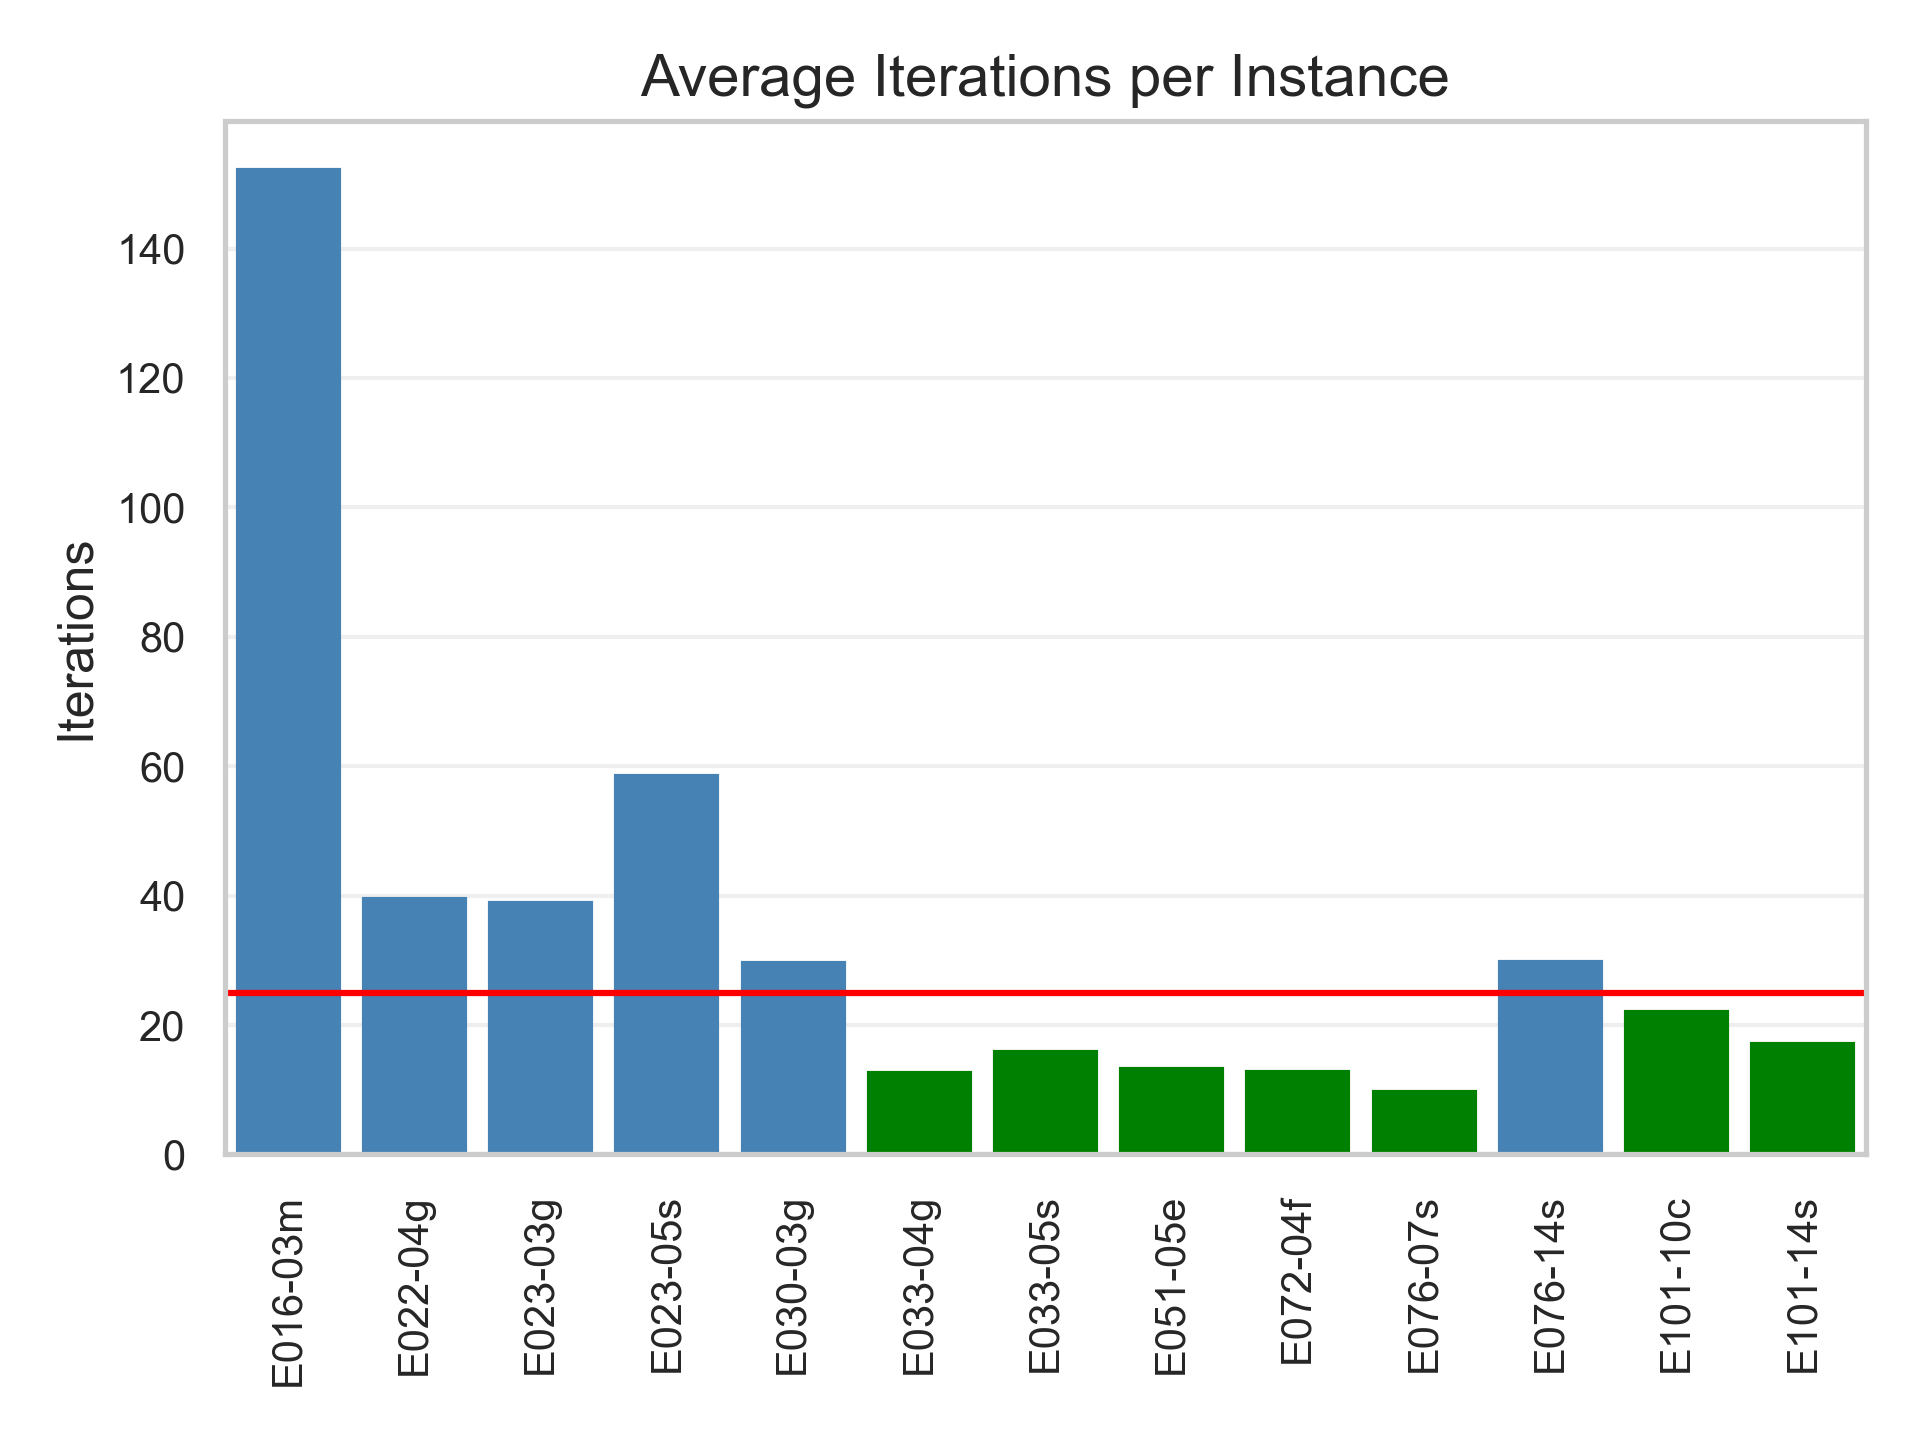
\includegraphics[width=\linewidth]{pictures/iterations_per_instance.png}
        \captionof{figure}{\small Average iterations for each \gendreauDataSetText instance.}
        \label{fig:average_iterations_noclassifier}
    \end{minipage}\hfill
    \begin{minipage}[t]{0.49\textwidth}
        \centering
        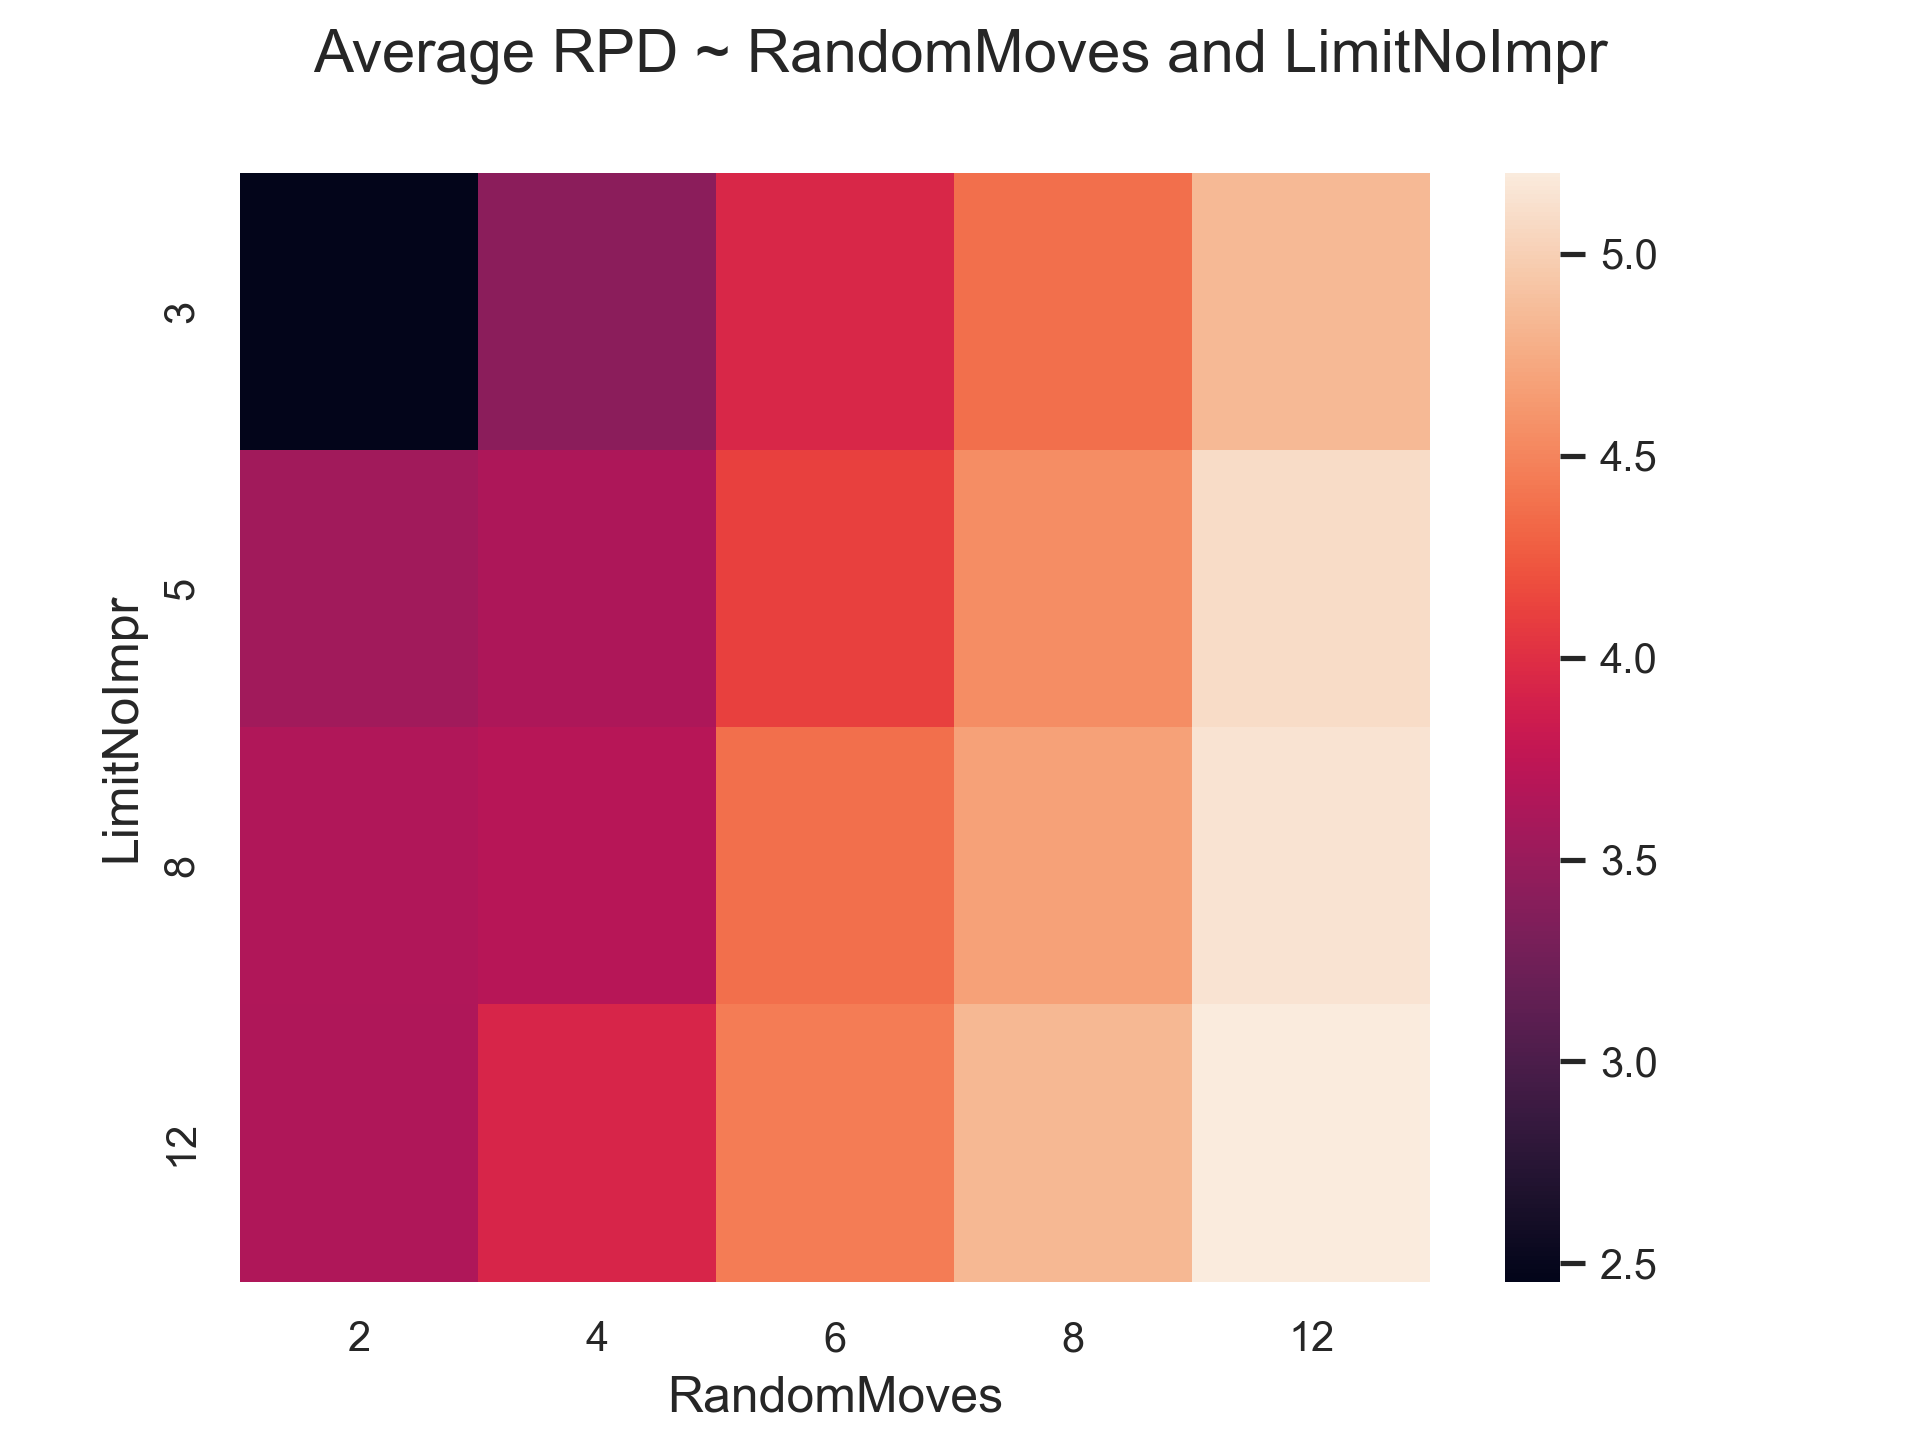
\includegraphics[width=\linewidth]{pictures/heatmap_randomMoves_limitNoImpr.png}
        \captionof{figure}{\small Dependency between RPD and RandomMoves and LimitNoImpr}
        \label{fig:heatmap_parameter_study}
    \end{minipage}
\end{figure}

The complete results are shown as boxplots for each parameter and performance metric in the Appendix Section~\ref{app:subsec:parameterstudy_noclassifier}.
This parameterstudy shows, that the order of the local search neighborhoods has the only significant effect and the inter neighborhoods
should be applied first (see Figure~\ref{fig:parameterstudy_NoClassifier_localSearch}). In general it can be observed again, that
the number of iterations matter most, as the results of the two groups introduced differ strongly performance wise. With these results
the parameters for the \gls{ILS} variants using the classifier can not be deduced, as the average number of iterations will be higher due to
speedups incorporated and the rejection rate plays a more significant role. For the comparison between the different variants the following
configuration will be chosen for NoClassifier:

\begin{table}[ht]
    \centering
    \begin{tabular}{@{}cccc@{}}
        \toprule
        AttemptsLimit & RandomMoves        R & Local Search order & Perturbation          \\
        \midrule
        3             & 4                    & InterLSFirst       & Both-Insertions-First \\
        \bottomrule
    \end{tabular}
    \caption{Final chosen parameters for the NoClassifier ILS variant.}
    \label{tab:parameters_final_noclassifier}
\end{table}

\subsection{SpeedUp Variant}
\label{subsec_parameterStuy_speedup}

\begin{table}[ht]
    \centering
    \begin{tabular}{c c }
        \toprule
        Parametertype            & Levels     \\
        \midrule
        IterationsWithoutCPCheck & [1,3,5,10] \\
        UseFilterStartSolution   & [1,0]      \\
        \bottomrule
    \end{tabular}
    \caption{Parameter levels for SpeedUp variant.}
    \label{tab:parameters_speedup}
\end{table}

\subsection{Hybrid Variant}
\label{subsec_parameterStuy_hybrid}

\begin{table}[ht]
    \centering
    \begin{tabular}{c c }
        \toprule
        Parametertype             & Levels                      \\
        \midrule
        Hybrid Usage Alternatives & \{[1,1,0],[1,0,1],[0,1,1]\} \\
        UseFilterStartSolution    & [1,0]                       \\
        \bottomrule
    \end{tabular}
    \caption{Parameter levels for hybrid variant.}
    \label{tab:parameters_hybrid}
\end{table}

\section{Comparison of heuristic variants}
\label{sec:comparison_ils_variants}

The solution quality for all four variants (see Fig.~\ref{fig:four_variants}) is compared by running all 27 instances.
The timelimit is in comparison to the parameterstudy now adapted by instance size. The following timelimits are identical
to \cite{zhang_evolutionary_2015}.\footcite[cf.][p.28]{zhang_evolutionary_2015}
\begin{table}[ht]
    \centering
    \begin{tabular}{C{0.24\linewidth}C{0.18\linewidth}C{0.18\linewidth}C{0.18\linewidth}}
        \toprule
        Customer number $N$ & $N \leq 25$ & $N < 25 < 50 $ & $N \geq 50 $ \\
        \midrule
        Timelimit [sec]     & 900         & 1800           & 3600         \\
        \bottomrule
    \end{tabular}
    \caption{Timelimit for the final heuristic comparisons.}
\end{table}

\section{Krebs will be cooked}
\label{sec:application_krebs}